\documentclass[]{article}
\usepackage{lmodern}
\usepackage{amssymb,amsmath}
\usepackage{ifxetex,ifluatex}
\usepackage{fixltx2e} % provides \textsubscript
\ifnum 0\ifxetex 1\fi\ifluatex 1\fi=0 % if pdftex
  \usepackage[T1]{fontenc}
  \usepackage[utf8]{inputenc}
\else % if luatex or xelatex
  \ifxetex
    \usepackage{mathspec}
  \else
    \usepackage{fontspec}
  \fi
  \defaultfontfeatures{Ligatures=TeX,Scale=MatchLowercase}
\fi
% use upquote if available, for straight quotes in verbatim environments
\IfFileExists{upquote.sty}{\usepackage{upquote}}{}
% use microtype if available
\IfFileExists{microtype.sty}{%
\usepackage{microtype}
\UseMicrotypeSet[protrusion]{basicmath} % disable protrusion for tt fonts
}{}
\usepackage[margin=1in]{geometry}
\usepackage{hyperref}
\hypersetup{unicode=true,
            pdftitle={Relative reliability of Models and variational Bayes},
            pdfborder={0 0 0},
            breaklinks=true}
\urlstyle{same}  % don't use monospace font for urls
\usepackage{color}
\usepackage{fancyvrb}
\newcommand{\VerbBar}{|}
\newcommand{\VERB}{\Verb[commandchars=\\\{\}]}
\DefineVerbatimEnvironment{Highlighting}{Verbatim}{commandchars=\\\{\}}
% Add ',fontsize=\small' for more characters per line
\usepackage{framed}
\definecolor{shadecolor}{RGB}{248,248,248}
\newenvironment{Shaded}{\begin{snugshade}}{\end{snugshade}}
\newcommand{\KeywordTok}[1]{\textcolor[rgb]{0.13,0.29,0.53}{\textbf{{#1}}}}
\newcommand{\DataTypeTok}[1]{\textcolor[rgb]{0.13,0.29,0.53}{{#1}}}
\newcommand{\DecValTok}[1]{\textcolor[rgb]{0.00,0.00,0.81}{{#1}}}
\newcommand{\BaseNTok}[1]{\textcolor[rgb]{0.00,0.00,0.81}{{#1}}}
\newcommand{\FloatTok}[1]{\textcolor[rgb]{0.00,0.00,0.81}{{#1}}}
\newcommand{\ConstantTok}[1]{\textcolor[rgb]{0.00,0.00,0.00}{{#1}}}
\newcommand{\CharTok}[1]{\textcolor[rgb]{0.31,0.60,0.02}{{#1}}}
\newcommand{\SpecialCharTok}[1]{\textcolor[rgb]{0.00,0.00,0.00}{{#1}}}
\newcommand{\StringTok}[1]{\textcolor[rgb]{0.31,0.60,0.02}{{#1}}}
\newcommand{\VerbatimStringTok}[1]{\textcolor[rgb]{0.31,0.60,0.02}{{#1}}}
\newcommand{\SpecialStringTok}[1]{\textcolor[rgb]{0.31,0.60,0.02}{{#1}}}
\newcommand{\ImportTok}[1]{{#1}}
\newcommand{\CommentTok}[1]{\textcolor[rgb]{0.56,0.35,0.01}{\textit{{#1}}}}
\newcommand{\DocumentationTok}[1]{\textcolor[rgb]{0.56,0.35,0.01}{\textbf{\textit{{#1}}}}}
\newcommand{\AnnotationTok}[1]{\textcolor[rgb]{0.56,0.35,0.01}{\textbf{\textit{{#1}}}}}
\newcommand{\CommentVarTok}[1]{\textcolor[rgb]{0.56,0.35,0.01}{\textbf{\textit{{#1}}}}}
\newcommand{\OtherTok}[1]{\textcolor[rgb]{0.56,0.35,0.01}{{#1}}}
\newcommand{\FunctionTok}[1]{\textcolor[rgb]{0.00,0.00,0.00}{{#1}}}
\newcommand{\VariableTok}[1]{\textcolor[rgb]{0.00,0.00,0.00}{{#1}}}
\newcommand{\ControlFlowTok}[1]{\textcolor[rgb]{0.13,0.29,0.53}{\textbf{{#1}}}}
\newcommand{\OperatorTok}[1]{\textcolor[rgb]{0.81,0.36,0.00}{\textbf{{#1}}}}
\newcommand{\BuiltInTok}[1]{{#1}}
\newcommand{\ExtensionTok}[1]{{#1}}
\newcommand{\PreprocessorTok}[1]{\textcolor[rgb]{0.56,0.35,0.01}{\textit{{#1}}}}
\newcommand{\AttributeTok}[1]{\textcolor[rgb]{0.77,0.63,0.00}{{#1}}}
\newcommand{\RegionMarkerTok}[1]{{#1}}
\newcommand{\InformationTok}[1]{\textcolor[rgb]{0.56,0.35,0.01}{\textbf{\textit{{#1}}}}}
\newcommand{\WarningTok}[1]{\textcolor[rgb]{0.56,0.35,0.01}{\textbf{\textit{{#1}}}}}
\newcommand{\AlertTok}[1]{\textcolor[rgb]{0.94,0.16,0.16}{{#1}}}
\newcommand{\ErrorTok}[1]{\textcolor[rgb]{0.64,0.00,0.00}{\textbf{{#1}}}}
\newcommand{\NormalTok}[1]{{#1}}
\usepackage{graphicx,grffile}
\makeatletter
\def\maxwidth{\ifdim\Gin@nat@width>\linewidth\linewidth\else\Gin@nat@width\fi}
\def\maxheight{\ifdim\Gin@nat@height>\textheight\textheight\else\Gin@nat@height\fi}
\makeatother
% Scale images if necessary, so that they will not overflow the page
% margins by default, and it is still possible to overwrite the defaults
% using explicit options in \includegraphics[width, height, ...]{}
\setkeys{Gin}{width=\maxwidth,height=\maxheight,keepaspectratio}
\IfFileExists{parskip.sty}{%
\usepackage{parskip}
}{% else
\setlength{\parindent}{0pt}
\setlength{\parskip}{6pt plus 2pt minus 1pt}
}
\setlength{\emergencystretch}{3em}  % prevent overfull lines
\providecommand{\tightlist}{%
  \setlength{\itemsep}{0pt}\setlength{\parskip}{0pt}}
\setcounter{secnumdepth}{0}
% Redefines (sub)paragraphs to behave more like sections
\ifx\paragraph\undefined\else
\let\oldparagraph\paragraph
\renewcommand{\paragraph}[1]{\oldparagraph{#1}\mbox{}}
\fi
\ifx\subparagraph\undefined\else
\let\oldsubparagraph\subparagraph
\renewcommand{\subparagraph}[1]{\oldsubparagraph{#1}\mbox{}}
\fi

%%% Use protect on footnotes to avoid problems with footnotes in titles
\let\rmarkdownfootnote\footnote%
\def\footnote{\protect\rmarkdownfootnote}

%%% Change title format to be more compact
\usepackage{titling}

% Create subtitle command for use in maketitle
\newcommand{\subtitle}[1]{
  \posttitle{
    \begin{center}\large#1\end{center}
    }
}

\setlength{\droptitle}{-2em}
  \title{Relative reliability of Models and variational Bayes}
  \pretitle{\vspace{\droptitle}\centering\huge}
  \posttitle{\par}
  \author{}
  \preauthor{}\postauthor{}
  \date{}
  \predate{}\postdate{}


\begin{document}
\maketitle

I am working on using a Bayesian model to estimate parameters for our
reward learning data. I'm extending
\href{https://rpubs.com/CCSL/hBayesDM}{Nate Haines' Double Update Model
for Reversal Learning}. Nate modified the version available in his
package hBayesDM to work with our dataset, which is a deterministic
Reversal Learning task. I have since incrementally extended it to handle
two different tasks (reward and punishment learning) and repeated runs.

In the latest, repeated runs version,
\texttt{double\_update\_rpo\_repeated\_runs}, I am getting values that
are quite different to earlier versions. There two possible explanations
I have for this:

\begin{itemize}
\tightlist
\item
  Either the former or current model isn't well designed. One or the
  other isn't reliable. The difference between the two is consistently
  inconsistent. We need to work out which is mis-specified.
\item
  Variational Bayes gives us different results each time we run the same
  model. Variational Bayes is known to be less precise (but faster) than
  Monte Carlo Markov Chain estimation.
\end{itemize}

These need to be tested out! So what we need to do is:

\begin{itemize}
\tightlist
\item
  run the models twice each
\item
  save values
\item
  compare Run1 mu, alpha, beta values for G2RiskyNoMeth and G3RiskyMeth
\end{itemize}

\subsection{Method}\label{method}

The hard part is running the model! This is done here. Let's compare:

\begin{itemize}
\tightlist
\item
  \texttt{double\_update\_rpo\_repeated\_runs.stan}, the latest model
  designed for multiple runs
\item
  \texttt{double\_update\_rp\_erroneous.stan}, processes reward and
  punishment data but only one run; there was an error that confused
  reward inverse temperature variance with punishment learning rate
  variance; I've included that here so we can compare to the resutls we
  obtained before the error was discovered.
\item
  \texttt{double\_update\_rp\_fixed.stan}, as above, but with the error
  fixed.
\item
  \texttt{double\_update.stan}, Processes only reward \emph{or}
  punishment data.
\end{itemize}

We also want to run several times.

\begin{Shaded}
\begin{Highlighting}[]
\NormalTok{models_to_run <-}\StringTok{ }\KeywordTok{c}\NormalTok{(}\StringTok{"double_update_rpo_repeated_runs"}\NormalTok{, }\StringTok{"double_update_rp_fixed"}\NormalTok{, }
    \StringTok{"double_update_rp_erroneous"}\NormalTok{, }\StringTok{"double_update"}\NormalTok{)}
\NormalTok{times_to_run =}\StringTok{ }\DecValTok{3}
\end{Highlighting}
\end{Shaded}

The run-wrapper now takes a ``file suffix'' which means we can run it
multiple times, each time with a different suffix, and the run will be
saved and given an appropriate name.

As we run these we need to be careful not to use up too much memory. We
probably ought to extract \emph{just the values we need}, which would
exclude the individual subject values, then take each object out of
memory.

\begin{Shaded}
\begin{Highlighting}[]
\NormalTok{if (}\KeywordTok{file.exists}\NormalTok{(}\StringTok{"model-summaries.RData"}\NormalTok{)) \{}
    \KeywordTok{load}\NormalTok{(}\DataTypeTok{file =} \StringTok{"model-summaries.RData"}\NormalTok{)}
\NormalTok{\} else \{}
    \NormalTok{model.summaries <-}\StringTok{ }\KeywordTok{vector}\NormalTok{(}\StringTok{"list"}\NormalTok{, }\DecValTok{2} \NormalTok{*}\StringTok{ }\KeywordTok{length}\NormalTok{(models_to_run) *}\StringTok{ }\NormalTok{times_to_run)}
\NormalTok{\}}

\NormalTok{if (}\KeywordTok{any}\NormalTok{(}\KeywordTok{sapply}\NormalTok{(model.summaries, is.null))) \{}
    \NormalTok{for (g in }\DecValTok{2}\NormalTok{:}\DecValTok{3}\NormalTok{) \{}
        \NormalTok{for (m in models_to_run) \{}
            \NormalTok{for (t in }\DecValTok{1}\NormalTok{:times_to_run) \{}
                \KeywordTok{print}\NormalTok{(}\KeywordTok{paste0}\NormalTok{(g, m, t, }\DataTypeTok{collapse =} \StringTok{", "}\NormalTok{))}
                \CommentTok{# only run reward and punishment when we can}
                \NormalTok{if (models_to_run %in%}\StringTok{ }\KeywordTok{c}\NormalTok{(}\StringTok{"double_update_rpo_repeated_runs"}\NormalTok{, }
                  \StringTok{"double_update_rp_fixed"}\NormalTok{, }\StringTok{"double_update_rp_erroneous"}\NormalTok{)) \{}
                  \NormalTok{rp <-}\StringTok{ }\KeywordTok{c}\NormalTok{(}\DecValTok{1}\NormalTok{, }\DecValTok{2}\NormalTok{)}
                \NormalTok{\} else \{}
                  \NormalTok{rp <-}\StringTok{ }\KeywordTok{c}\NormalTok{(}\DecValTok{2}\NormalTok{)}
                \NormalTok{\}}
                \CommentTok{# only run multiple runs when we can}
                \NormalTok{if (models_to_run %in%}\StringTok{ }\KeywordTok{c}\NormalTok{(}\StringTok{"double_update_rpo_repeated_runs"}\NormalTok{)) \{}
                  \NormalTok{runs =}\StringTok{ }\KeywordTok{c}\NormalTok{(}\DecValTok{1}\NormalTok{, }\DecValTok{2}\NormalTok{)}
                  \NormalTok{generatePosteriorTrialPredictions =}\StringTok{ }\OtherTok{FALSE}
                \NormalTok{\} else \{}
                  \NormalTok{runs =}\StringTok{ }\KeywordTok{c}\NormalTok{(}\DecValTok{1}\NormalTok{)}
                  \NormalTok{generatePosteriorTrialPredictions =}\StringTok{ }\OtherTok{NA}
                \NormalTok{\}}
                \CommentTok{# run the model}
                \NormalTok{fit <-}\StringTok{ }\KeywordTok{lookupOrRunFit}\NormalTok{(}\DataTypeTok{run =} \NormalTok{runs, }\DataTypeTok{groups_to_fit =} \NormalTok{g, }\DataTypeTok{model_to_use =} \NormalTok{m, }
                  \DataTypeTok{includeSubjGroup =} \OtherTok{FALSE}\NormalTok{, }\DataTypeTok{rp =} \NormalTok{rp, }\DataTypeTok{model_rp_separately =} \OtherTok{TRUE}\NormalTok{, }
                  \DataTypeTok{model_runs_separately =} \OtherTok{TRUE}\NormalTok{, }\DataTypeTok{include_pain =} \OtherTok{FALSE}\NormalTok{, }\DataTypeTok{fileSuffix =} \KeywordTok{paste0}\NormalTok{(}\StringTok{"20170923_test_iteration_"}\NormalTok{, }
                    \KeywordTok{as.character}\NormalTok{(t), }\DataTypeTok{generatePosteriorTrialPredictions =} \NormalTok{generatePosteriorTrialPredictions))}
                
                \KeywordTok{cat}\NormalTok{(}\StringTok{"...model loaded. Extracting..."}\NormalTok{)}
                \CommentTok{# save just the output we want.}
                \NormalTok{first_empty_list_pos <-}\StringTok{ }\KeywordTok{min}\NormalTok{(}\KeywordTok{which}\NormalTok{(}\KeywordTok{sapply}\NormalTok{(model.summaries, is.null)))}
                \KeywordTok{print}\NormalTok{(}\KeywordTok{paste}\NormalTok{(}\StringTok{"first_empty_list_pos is"}\NormalTok{, }\KeywordTok{as.character}\NormalTok{(first_empty_list_pos)))}
                
                
                \NormalTok{if (m ==}\StringTok{ "double_update_rpo_repeated_runs"}\NormalTok{) \{}
                  \NormalTok{model.summaries[[first_empty_list_pos]] <-}\StringTok{ }\KeywordTok{list}\NormalTok{(}\DataTypeTok{summaryObj =} \KeywordTok{data_summarize_double_update_rpo_repeated_runs}\NormalTok{(rstan::}\KeywordTok{extract}\NormalTok{(fit$fit)), }
                    \DataTypeTok{g =} \NormalTok{g, }\DataTypeTok{m =} \NormalTok{m, }\DataTypeTok{t =} \NormalTok{t)}
                \NormalTok{\} else if (m ==}\StringTok{ "double_update_rp_erroneous"} \NormalTok{||}\StringTok{ }\NormalTok{m ==}\StringTok{ "double_update_rp_fixed"}\NormalTok{) \{}
                  \NormalTok{model.summaries[[first_empty_list_pos]] <-}\StringTok{ }\KeywordTok{list}\NormalTok{(}\DataTypeTok{summaryObj =} \KeywordTok{data_summarize_double_update_rp}\NormalTok{(rstan::}\KeywordTok{extract}\NormalTok{(fit$fit), }
                    \DataTypeTok{run =} \NormalTok{runs), }\DataTypeTok{g =} \NormalTok{g, }\DataTypeTok{m =} \NormalTok{m, }\DataTypeTok{t =} \NormalTok{t)}
                \NormalTok{\} else if (m ==}\StringTok{ "double_update"}\NormalTok{) \{}
                  \NormalTok{model.summaries[[first_empty_list_pos]] <-}\StringTok{ }\KeywordTok{list}\NormalTok{(}\DataTypeTok{summaryObj =} \KeywordTok{data_summarize_double_update}\NormalTok{(rstan::}\KeywordTok{extract}\NormalTok{(fit$fit), }
                    \DataTypeTok{outcome.type =} \NormalTok{rp, }\DataTypeTok{run =} \NormalTok{runs), }\DataTypeTok{g =} \NormalTok{g, }\DataTypeTok{m =} \NormalTok{m, }\DataTypeTok{t =} \NormalTok{t)}
                \NormalTok{\} else \{}
                  \KeywordTok{stop}\NormalTok{(}\StringTok{"f^<%! I don't recognize that model."}\NormalTok{)}
                \NormalTok{\}}
                \CommentTok{# remove the fit object from memory, because it is pretty large!}
                \KeywordTok{rm}\NormalTok{(fit)}
                \KeywordTok{print}\NormalTok{(}\StringTok{"...summary data extracted."}\NormalTok{)}
            \NormalTok{\}}
        \NormalTok{\}}
    \NormalTok{\}}
    \KeywordTok{save}\NormalTok{(model.summaries, }\DataTypeTok{file =} \StringTok{"model-summaries.RData"}\NormalTok{)}
\NormalTok{\}}
\end{Highlighting}
\end{Shaded}

\subsection{Results}\label{results}

For each of the four models, we can compare to see how closely analyses
runs matched one another. For each of the Run1 mu, sigma, alpha, beta
values for G2RiskyNoMeth and G3RiskyMeth, we can see how much variance
exists within and how much variance exists between models.

\begin{Shaded}
\begin{Highlighting}[]
\CommentTok{# arrange all the data into a single data table.}
\NormalTok{model.summary.all <-}\StringTok{ }\OtherTok{NULL}
\NormalTok{for (ms in model.summaries) \{}
    \NormalTok{ms.summaryObj <-}\StringTok{ }\NormalTok{ms$summaryObj}
    \NormalTok{ms.summaryObj$Group <-}\StringTok{ }\NormalTok{ms$g}
    \NormalTok{ms.summaryObj$ModelName <-}\StringTok{ }\NormalTok{ms$m}
    \NormalTok{ms.summaryObj$AnalysisRepetition <-}\StringTok{ }\NormalTok{ms$t}
    \NormalTok{if (}\KeywordTok{is.null}\NormalTok{(model.summary.all)) \{}
        \NormalTok{model.summary.all <-}\StringTok{ }\NormalTok{ms.summaryObj}
    \NormalTok{\} else \{}
        \NormalTok{model.summary.all <-}\StringTok{ }\KeywordTok{rbind}\NormalTok{(model.summary.all, ms.summaryObj)}
    \NormalTok{\}}
\NormalTok{\}}
\end{Highlighting}
\end{Shaded}

\subsubsection{Alpha mu (learning rate)}\label{alpha-mu-learning-rate}

\begin{verbatim}
##                               Df Sum Sq Mean Sq  F value   Pr(>F)    
## factor(AnalysisRepetition)     2  0.094   0.047    28.32 5.32e-13 ***
## factor(Group)                  1 26.309  26.309 15902.67  < 2e-16 ***
## ModelName                      3  2.508   0.836   505.33  < 2e-16 ***
## Residuals                  14963 24.754   0.002                      
## ---
## Signif. codes:  0 '***' 0.001 '**' 0.01 '*' 0.05 '.' 0.1 ' ' 1
\end{verbatim}

\begin{verbatim}
## Single term deletions
## 
## Model:
## Value ~ factor(AnalysisRepetition) + factor(Group) + ModelName
##                            Df Sum of Sq    RSS    AIC   F value    Pr(>F)
## <none>                                  24.754 -95866                    
## factor(AnalysisRepetition)  2    0.0937 24.848 -95813    28.316 5.321e-13
## factor(Group)               1   26.3088 51.063 -85029 15902.675 < 2.2e-16
## ModelName                   3    2.5080 27.262 -94427   505.327 < 2.2e-16
##                               
## <none>                        
## factor(AnalysisRepetition) ***
## factor(Group)              ***
## ModelName                  ***
## ---
## Signif. codes:  0 '***' 0.001 '**' 0.01 '*' 0.05 '.' 0.1 ' ' 1
\end{verbatim}

It appears that repetition did make a difference, but most of the
variance here really does seem to be in the model name (and even more
between groups!)

\subsubsection{Beta mu (inverse
temperature)}\label{beta-mu-inverse-temperature}

\begin{verbatim}
##                               Df Sum Sq Mean Sq F value Pr(>F)    
## factor(AnalysisRepetition)     2   2.41    1.21   195.7 <2e-16 ***
## factor(Group)                  1  57.86   57.86  9390.1 <2e-16 ***
## ModelName                      3   7.80    2.60   422.1 <2e-16 ***
## Residuals                  14963  92.19    0.01                   
## ---
## Signif. codes:  0 '***' 0.001 '**' 0.01 '*' 0.05 '.' 0.1 ' ' 1
\end{verbatim}

\begin{verbatim}
## Single term deletions
## 
## Model:
## Value ~ factor(AnalysisRepetition) + factor(Group) + ModelName
##                            Df Sum of Sq     RSS    AIC F value    Pr(>F)
## <none>                                   92.194 -76182                  
## factor(AnalysisRepetition)  2     2.411  94.605 -75799  195.68 < 2.2e-16
## factor(Group)               1    57.856 150.050 -68892 9390.07 < 2.2e-16
## ModelName                   3     7.803  99.997 -74972  422.14 < 2.2e-16
##                               
## <none>                        
## factor(AnalysisRepetition) ***
## factor(Group)              ***
## ModelName                  ***
## ---
## Signif. codes:  0 '***' 0.001 '**' 0.01 '*' 0.05 '.' 0.1 ' ' 1
\end{verbatim}

We can visualize how that looks.

\begin{Shaded}
\begin{Highlighting}[]
\KeywordTok{source}\NormalTok{(}\StringTok{"../visualization/geom_hdi.R"}\NormalTok{)}

\NormalTok{m.reward.mu.run1 <-}\StringTok{ }\NormalTok{model.summary.all[Motivation ==}\StringTok{ "Reward"} \NormalTok{&}\StringTok{ }\NormalTok{Statistic ==}\StringTok{ }
\StringTok{    "mu"} \NormalTok{&}\StringTok{ }\NormalTok{Run ==}\StringTok{ }\DecValTok{1}\NormalTok{]}
\CommentTok{# table(m.reward.mu.run1$ModelName) for clarity's sake...}
\NormalTok{m.reward.mu.run1$ModelName <-}\StringTok{ }\KeywordTok{sub}\NormalTok{(}\StringTok{"double_update"}\NormalTok{, }\StringTok{"DU"}\NormalTok{, m.reward.mu.run1$ModelName)}

\CommentTok{# plotly::ggplotly(p)}
\KeywordTok{ggplot}\NormalTok{(m.reward.mu.run1[Parameter ==}\StringTok{ "alpha"}\NormalTok{], }\KeywordTok{aes}\NormalTok{(}\DataTypeTok{x =} \NormalTok{Value, }\DataTypeTok{fill =} \KeywordTok{factor}\NormalTok{(Group), }
    \DataTypeTok{color =} \KeywordTok{factor}\NormalTok{(Group))) +}\StringTok{ }\KeywordTok{geom_freqpoly}\NormalTok{(}\DataTypeTok{alpha =} \FloatTok{0.9}\NormalTok{, }\DataTypeTok{binwidth =} \FloatTok{0.001}\NormalTok{) +}\StringTok{ }
\StringTok{    }\KeywordTok{geom_hdi}\NormalTok{(}\DataTypeTok{size =} \DecValTok{2}\NormalTok{, }\DataTypeTok{lineend =} \StringTok{"round"}\NormalTok{, }\DataTypeTok{alpha =} \FloatTok{0.5}\NormalTok{, }\DataTypeTok{credible_mass =} \FloatTok{0.95}\NormalTok{) +}\StringTok{ }
\StringTok{    }\KeywordTok{facet_grid}\NormalTok{(ModelName ~}\StringTok{ }\NormalTok{AnalysisRepetition) +}\StringTok{ }\KeywordTok{labs}\NormalTok{(}\DataTypeTok{title =} \KeywordTok{paste0}\NormalTok{(}\StringTok{"mu statistic in reward rounds, alpha"}\NormalTok{))}
\end{Highlighting}
\end{Shaded}

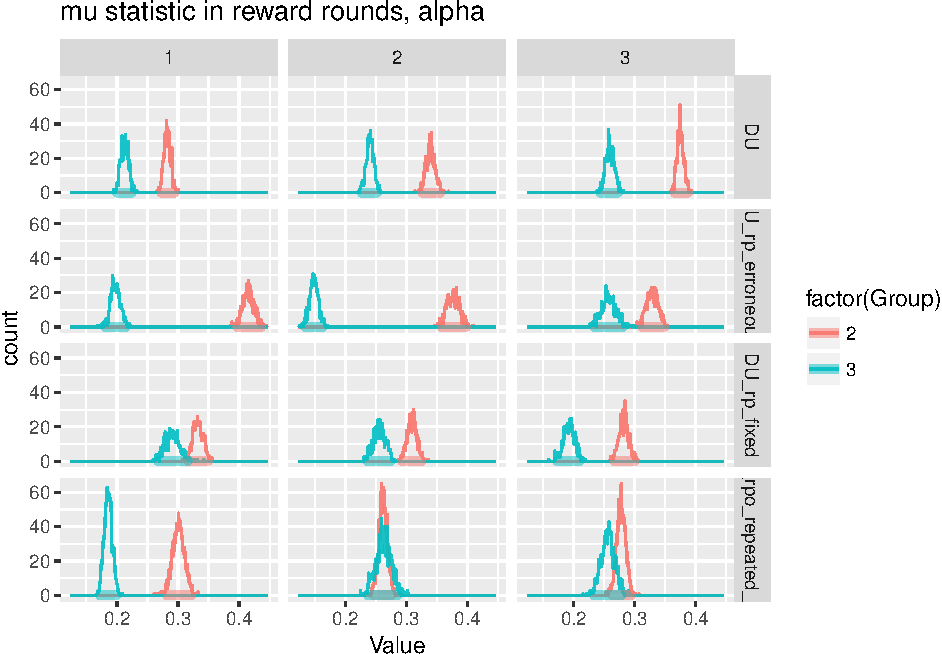
\includegraphics{compare_models_files/figure-latex/AOVVisualize-1.pdf}

\begin{verbatim}
## [1] 0.272950 0.294087
## [1] 0.200155 0.224060
## [1] 0.326095 0.355326
## [1] 0.227055 0.251767
## [1] 0.365537 0.387050
## [1] 0.244250 0.272503
## [1] 0.397188 0.435854
## [1] 0.181596 0.213906
## [1] 0.357979 0.397369
## [1] 0.134462 0.163076
## [1] 0.312867 0.348189
## [1] 0.234208 0.280359
## [1] 0.317159 0.348665
## [1] 0.267506 0.315760
## [1] 0.293319 0.323937
## [1] 0.237153 0.274108
## [1] 0.267363 0.299793
## [1] 0.173228 0.209031
## [1] 0.282781 0.321303
## [1] 0.172944 0.198344
## [1] 0.246633 0.275435
## [1] 0.237643 0.285343
## [1] 0.264587 0.293882
## [1] 0.234070 0.277762
\end{verbatim}

\begin{Shaded}
\begin{Highlighting}[]
\KeywordTok{ggplot}\NormalTok{(m.reward.mu.run1[Parameter ==}\StringTok{ "beta"}\NormalTok{], }\KeywordTok{aes}\NormalTok{(}\DataTypeTok{x =} \NormalTok{Value, }\DataTypeTok{fill =} \KeywordTok{factor}\NormalTok{(Group), }
    \DataTypeTok{color =} \KeywordTok{factor}\NormalTok{(Group))) +}\StringTok{ }\KeywordTok{geom_freqpoly}\NormalTok{(}\DataTypeTok{alpha =} \FloatTok{0.9}\NormalTok{, }\DataTypeTok{binwidth =} \FloatTok{0.001}\NormalTok{) +}\StringTok{ }
\StringTok{    }\KeywordTok{geom_hdi}\NormalTok{(}\DataTypeTok{size =} \DecValTok{2}\NormalTok{, }\DataTypeTok{lineend =} \StringTok{"round"}\NormalTok{, }\DataTypeTok{alpha =} \FloatTok{0.9}\NormalTok{, }\DataTypeTok{credible_mass =} \FloatTok{0.95}\NormalTok{) +}\StringTok{ }
\StringTok{    }\KeywordTok{facet_grid}\NormalTok{(ModelName ~}\StringTok{ }\NormalTok{AnalysisRepetition) +}\StringTok{ }\KeywordTok{labs}\NormalTok{(}\DataTypeTok{title =} \KeywordTok{paste0}\NormalTok{(}\StringTok{"mu statistic in reward rounds, beta"}\NormalTok{))}
\end{Highlighting}
\end{Shaded}

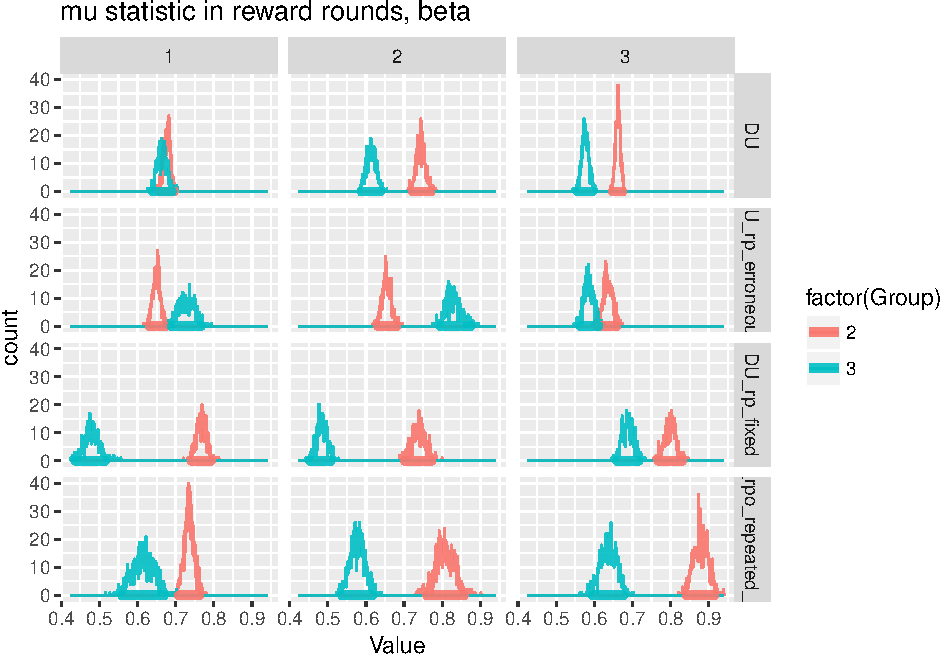
\includegraphics{compare_models_files/figure-latex/AOVVisualize-2.pdf}

\begin{verbatim}
## [1] 0.658596 0.694864
## [1] 0.640187 0.689322
## [1] 0.723227 0.769291
## [1] 0.588819 0.637108
## [1] 0.648828 0.673521
## [1] 0.557232 0.594427
## [1] 0.631726 0.672060
## [1] 0.69031 0.76547
## [1] 0.632034 0.679211
## [1] 0.796454 0.874416
## [1] 0.607673 0.658229
## [1] 0.564077 0.610909
## [1] 0.741543 0.792076
## [1] 0.437816 0.514460
## [1] 0.702171 0.771998
## [1] 0.453951 0.507808
## [1] 0.767843 0.830039
## [1] 0.659766 0.715835
## [1] 0.708693 0.761434
## [1] 0.560357 0.668903
## [1] 0.761130 0.856477
## [1] 0.537677 0.616680
## [1] 0.842301 0.914251
## [1] 0.595638 0.675780
\end{verbatim}

There is one thing consistent across all samples for the reward round,
no matter what model is used and across both repetitions. Meth users
have lower or similar learning rates compared to Non-users. In no runs
did we find that meth users had higher learning rates or inverse
temperatures than non-users.

However, there is considerable variation across both runs and models.
Importantly, for the final model, which takes into account Run2 and also
calculates both reward and punishment, posterior alpha (learning rate)
samples overlapped such that it is visually not clear there was a
significant difference between groups. If we examine the difference
between groups for each analysis, we can see that the 95\% HDI includes
(and in fact, is pretty closely centered around) zero for two of the
three analyses run for the final model.

\begin{Shaded}
\begin{Highlighting}[]
\NormalTok{alpha_lastModel <-}\StringTok{ }\NormalTok{tidyr::}\KeywordTok{spread}\NormalTok{(m.reward.mu.run1[Parameter ==}\StringTok{ "alpha"} \NormalTok{&}\StringTok{ }\NormalTok{ModelName ==}\StringTok{ }
\StringTok{    "DU_rpo_repeated_runs"}\NormalTok{], Group, Value)}

\NormalTok{alpha_lastModel$GroupDifference <-}\StringTok{ }\NormalTok{alpha_lastModel$}\StringTok{`}\DataTypeTok{2}\StringTok{`} \NormalTok{-}\StringTok{ }\NormalTok{alpha_lastModel$}\StringTok{`}\DataTypeTok{3}\StringTok{`}

\NormalTok{lastModelPlot <-}\StringTok{ }\KeywordTok{ggplot}\NormalTok{(alpha_lastModel, }\KeywordTok{aes}\NormalTok{(}\DataTypeTok{x =} \NormalTok{GroupDifference, }\DataTypeTok{color =} \KeywordTok{factor}\NormalTok{(AnalysisRepetition))) +}\StringTok{ }
\StringTok{    }\KeywordTok{geom_freqpoly}\NormalTok{(}\DataTypeTok{alpha =} \FloatTok{0.9}\NormalTok{, }\DataTypeTok{binwidth =} \FloatTok{0.001}\NormalTok{) +}\StringTok{ }\KeywordTok{geom_hdi}\NormalTok{(}\DataTypeTok{size =} \DecValTok{2}\NormalTok{, }\DataTypeTok{lineend =} \StringTok{"round"}\NormalTok{, }
    \DataTypeTok{alpha =} \FloatTok{0.5}\NormalTok{, }\DataTypeTok{credible_mass =} \FloatTok{0.95}\NormalTok{) +}\StringTok{ }\KeywordTok{labs}\NormalTok{(}\DataTypeTok{title =} \StringTok{"learning rate NoMeth-Meth group difference credible values, by Analysis}\CharTok{\textbackslash{}n}\StringTok{With 95% Highest Density Intervals"}\NormalTok{)}

\CommentTok{# plotly::ggplotly(lastModelPlot)}

\NormalTok{lastModelPlot}
\end{Highlighting}
\end{Shaded}

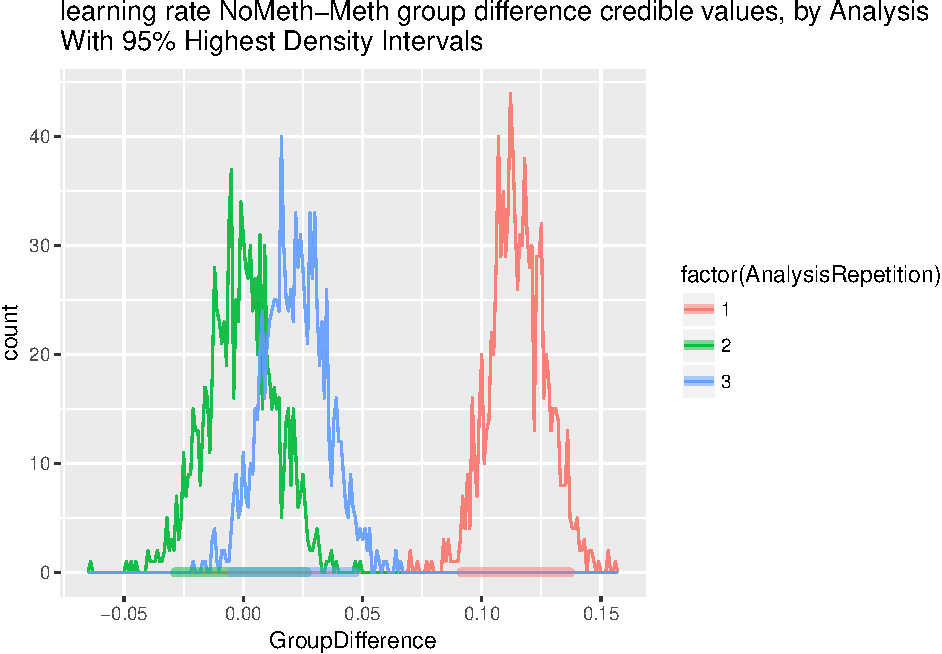
\includegraphics{compare_models_files/figure-latex/lastModelFollowup-1.pdf}

\begin{verbatim}
## [1] 0.091521 0.136928
## [1] -0.028491  0.026618
## [1] -0.004796  0.046774
\end{verbatim}

Differences between the groups varied considerably depending on whether
we examine Analysis Run 1 or Run 2. For the second analysis, there were
very small differences between groups; for the first analysis
differences seemed to be larger. There was also quite a lot of variation
between the parameters estimated by the different models, although it is
not clear that it is necessary to go to the model used to explain the
difference - this may simply be due to the random effects of each
analysis.

\subsection{Pairs plots}\label{pairs-plots}

Might be useful to know about the possible correlations between
variables. Let's take a look at a sample of four of the chains:

\begin{Shaded}
\begin{Highlighting}[]
\KeywordTok{library}\NormalTok{(GGally)}
\KeywordTok{source}\NormalTok{(}\StringTok{"../visualization/gg_labelledcormap.R"}\NormalTok{)}

\NormalTok{for (s in model.summaries}\CommentTok{#[(1:4)*length(model.summaries)/4]}
     \NormalTok{)\{}
  \NormalTok{summary.name<-}\KeywordTok{paste}\NormalTok{(}\StringTok{"group="}\NormalTok{,}\KeywordTok{as.character}\NormalTok{(s$g),}\StringTok{"m="}\NormalTok{,s$m,}\StringTok{"t="}\NormalTok{,}\KeywordTok{as.character}\NormalTok{(s$t))}
  \NormalTok{s.wide.all<-data.table::}\KeywordTok{dcast}\NormalTok{(}
    \DataTypeTok{data =} \NormalTok{s[[}\StringTok{"summaryObj"}\NormalTok{]],}
    \NormalTok{iter~Motivation+Run+Statistic+Parameter,}
    \DataTypeTok{value.var=}\StringTok{"Value"}
    \NormalTok{)}
  \NormalTok{s.wide<-s.wide.all[,}\DecValTok{2}\NormalTok{:(}\KeywordTok{dim}\NormalTok{(s.wide.all)[}\DecValTok{2}\NormalTok{]-}\DecValTok{1}\NormalTok{)]}
  \KeywordTok{colnames}\NormalTok{(s.wide)<-}\KeywordTok{gsub}\NormalTok{(}\StringTok{"diff"}\NormalTok{,}\StringTok{"Delta"}\NormalTok{,}\KeywordTok{gsub}\NormalTok{(}\StringTok{"_"}\NormalTok{,}\StringTok{"~"}\NormalTok{,}\KeywordTok{gsub}\NormalTok{(}\StringTok{"Reward_"}\NormalTok{,}\StringTok{"R~"}\NormalTok{,}\KeywordTok{gsub}\NormalTok{(}\StringTok{"Punishment_"}\NormalTok{,}\StringTok{"P~"}\NormalTok{,}\KeywordTok{colnames}\NormalTok{(s.wide)))))}
  \NormalTok{custom_ggpairs<-}\KeywordTok{ggpairs}\NormalTok{(s.wide,}\CommentTok{#dim(s.wide)[2]],}
                          \DataTypeTok{lower =} \KeywordTok{list}\NormalTok{(}\DataTypeTok{continuous =} \KeywordTok{wrap}\NormalTok{(}\StringTok{"points"}\NormalTok{, }\DataTypeTok{alpha =} \FloatTok{0.1}\NormalTok{,}\DataTypeTok{size=}\FloatTok{0.25}\NormalTok{)),}
                          \DataTypeTok{upper =} \KeywordTok{list}\NormalTok{(}\DataTypeTok{continuous =} \KeywordTok{wrap}\NormalTok{(}\StringTok{"cor"}\NormalTok{,}\DataTypeTok{size=}\DecValTok{2}\NormalTok{,}\DataTypeTok{color=}\StringTok{"blue"}\NormalTok{)),}
                          \DataTypeTok{columnLabels =} \KeywordTok{colnames}\NormalTok{(s.wide),}
                          \DataTypeTok{labeller =} \StringTok{"label_parsed"}\NormalTok{,}\DataTypeTok{title =} \NormalTok{summary.name)}
  \KeywordTok{print}\NormalTok{(custom_ggpairs)}

\NormalTok{\}}
\end{Highlighting}
\end{Shaded}

\includegraphics{compare_models_files/figure-latex/PairsPlots-1.pdf}
\includegraphics{compare_models_files/figure-latex/PairsPlots-2.pdf}
\includegraphics{compare_models_files/figure-latex/PairsPlots-3.pdf}
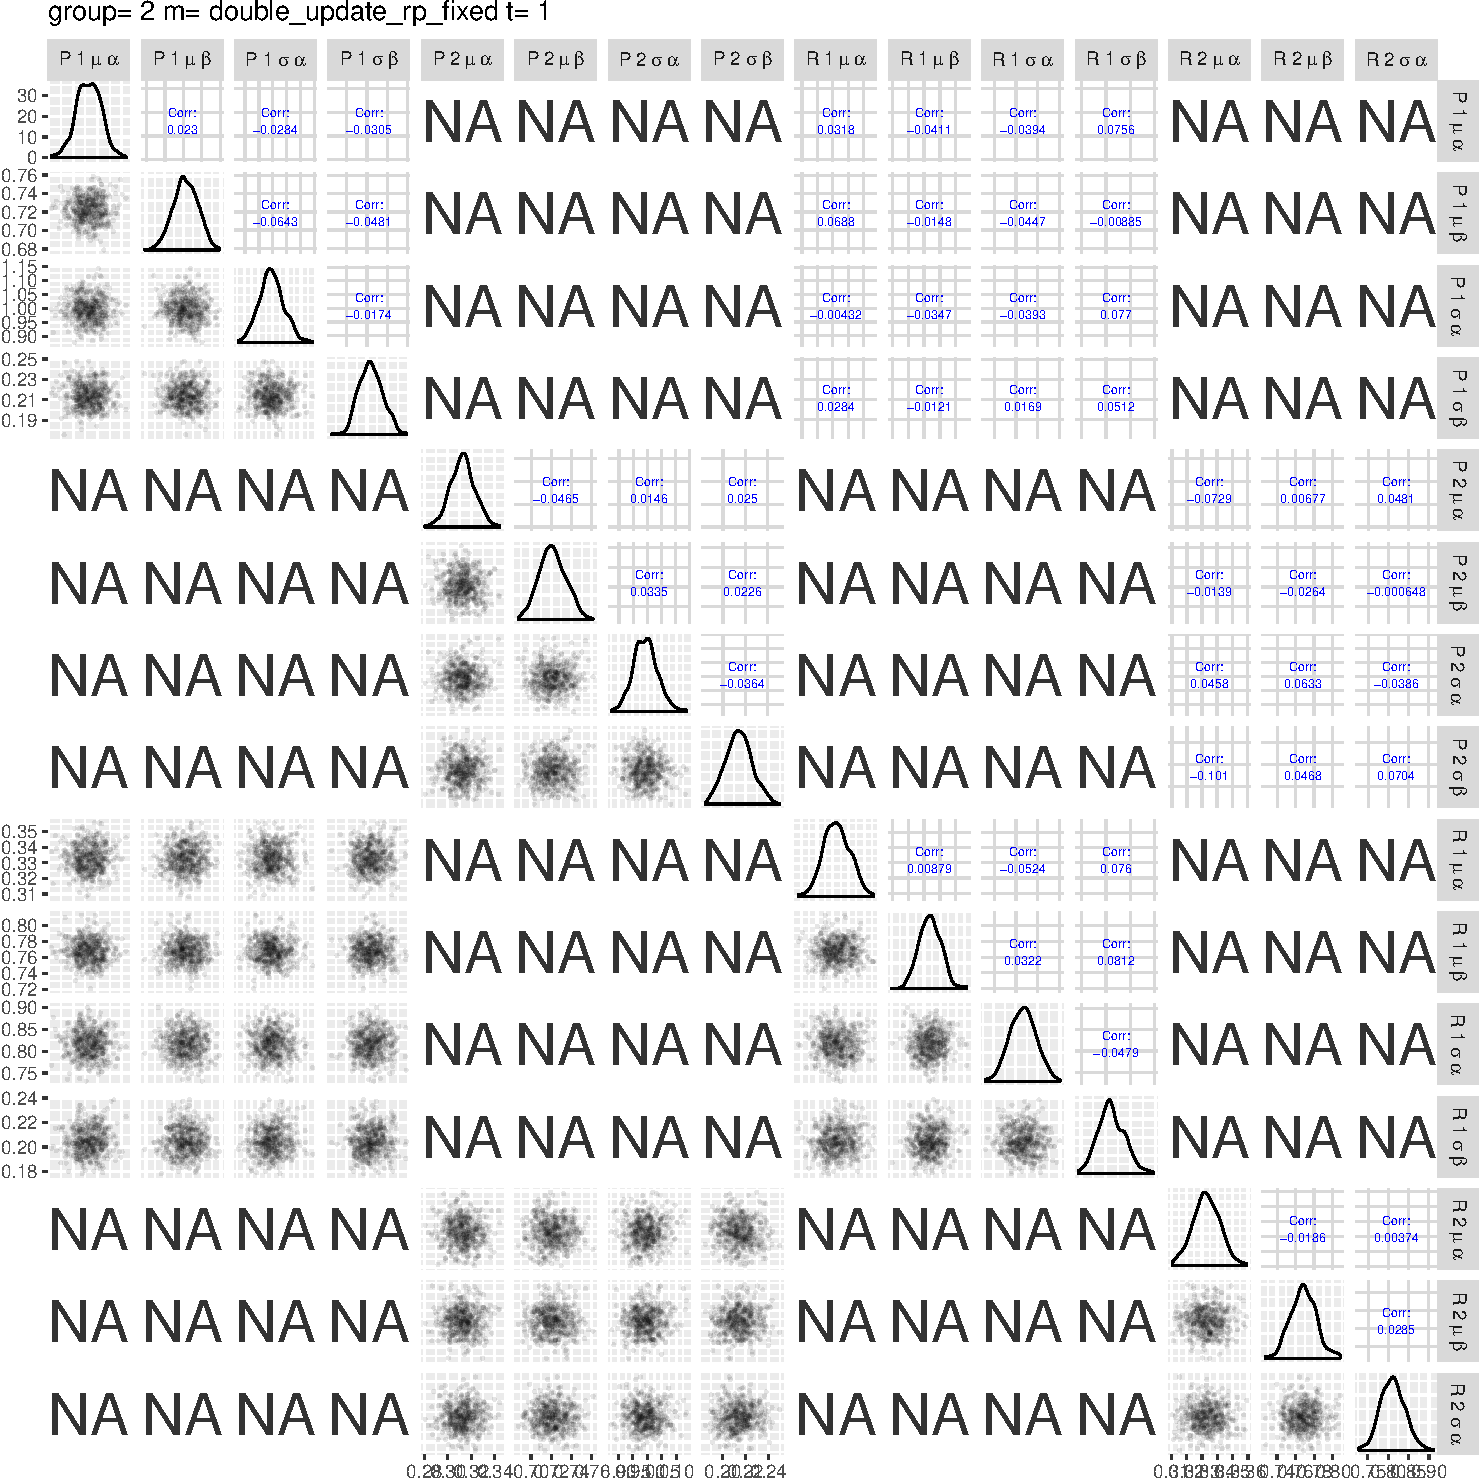
\includegraphics{compare_models_files/figure-latex/PairsPlots-4.pdf}
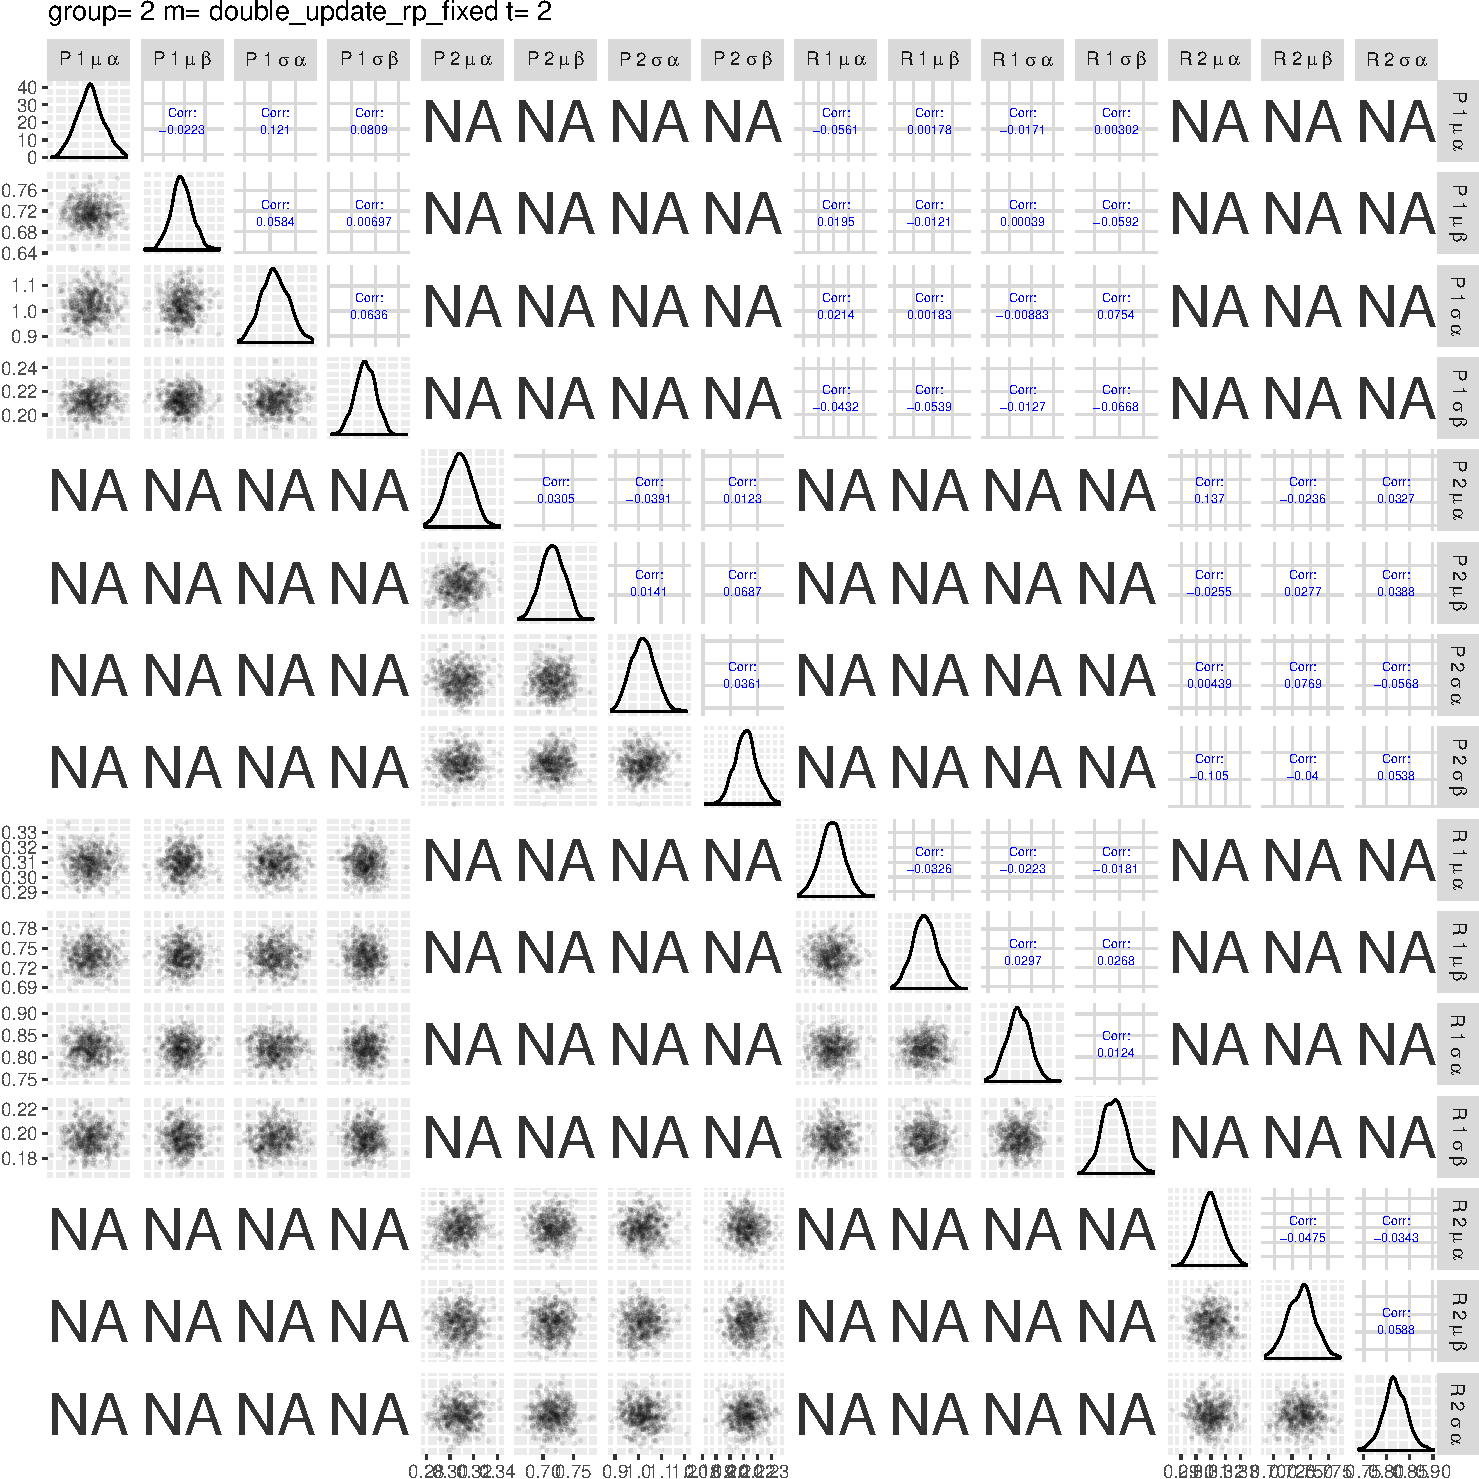
\includegraphics{compare_models_files/figure-latex/PairsPlots-5.pdf}
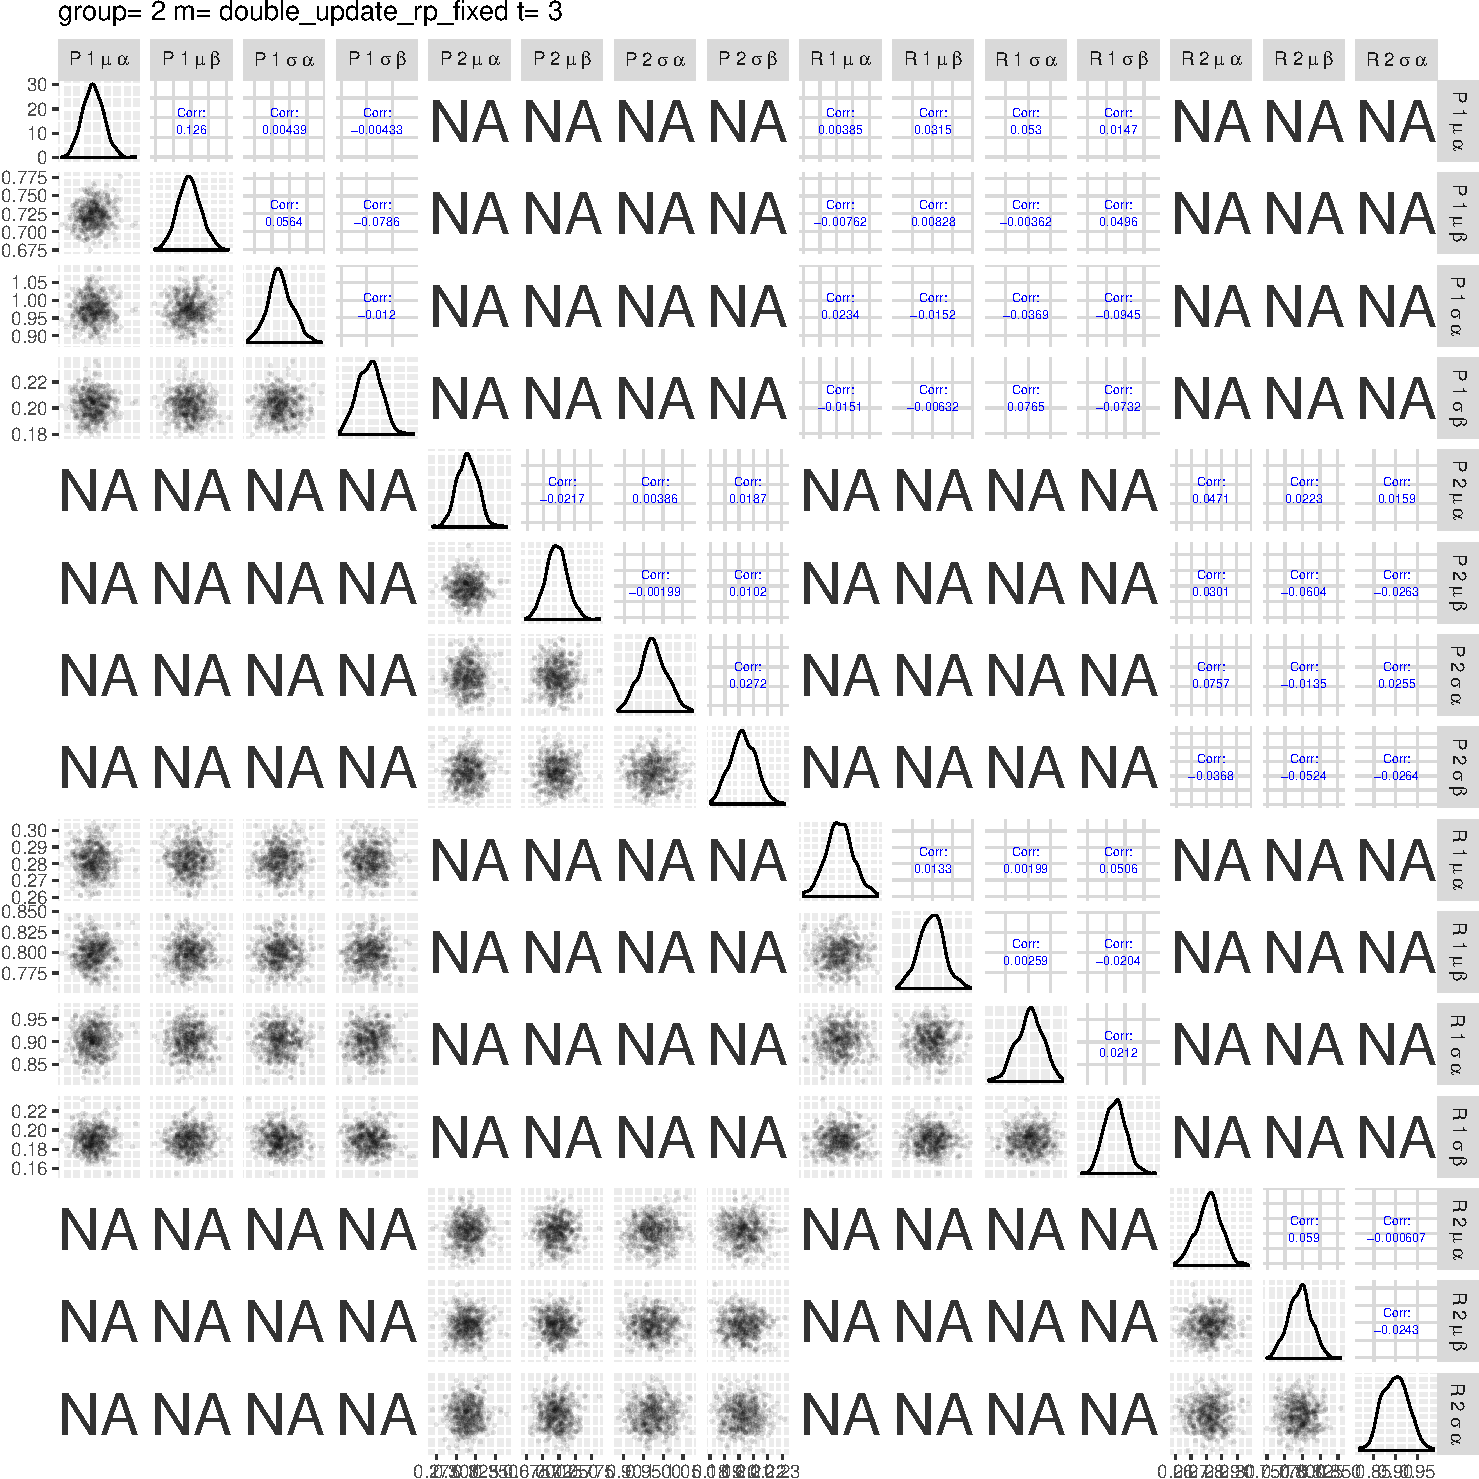
\includegraphics{compare_models_files/figure-latex/PairsPlots-6.pdf}
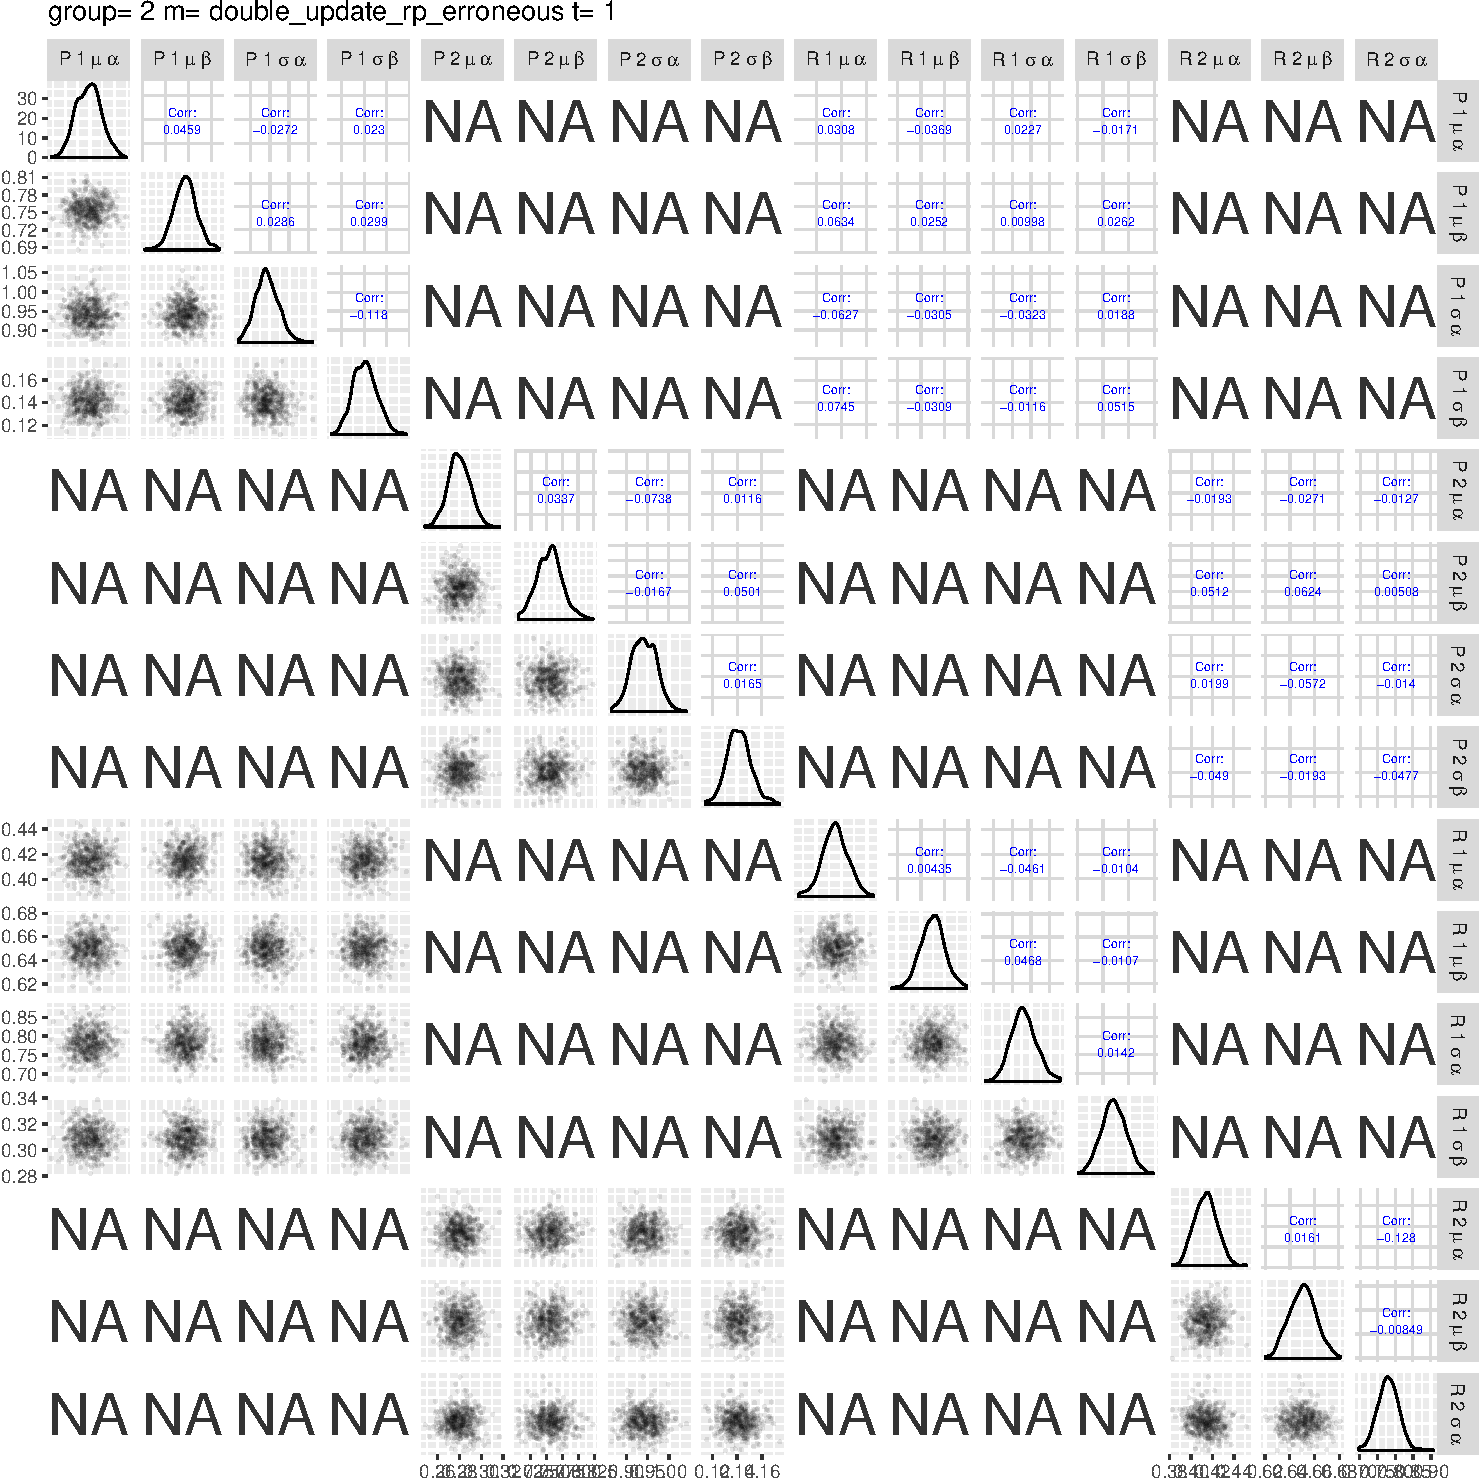
\includegraphics{compare_models_files/figure-latex/PairsPlots-7.pdf}
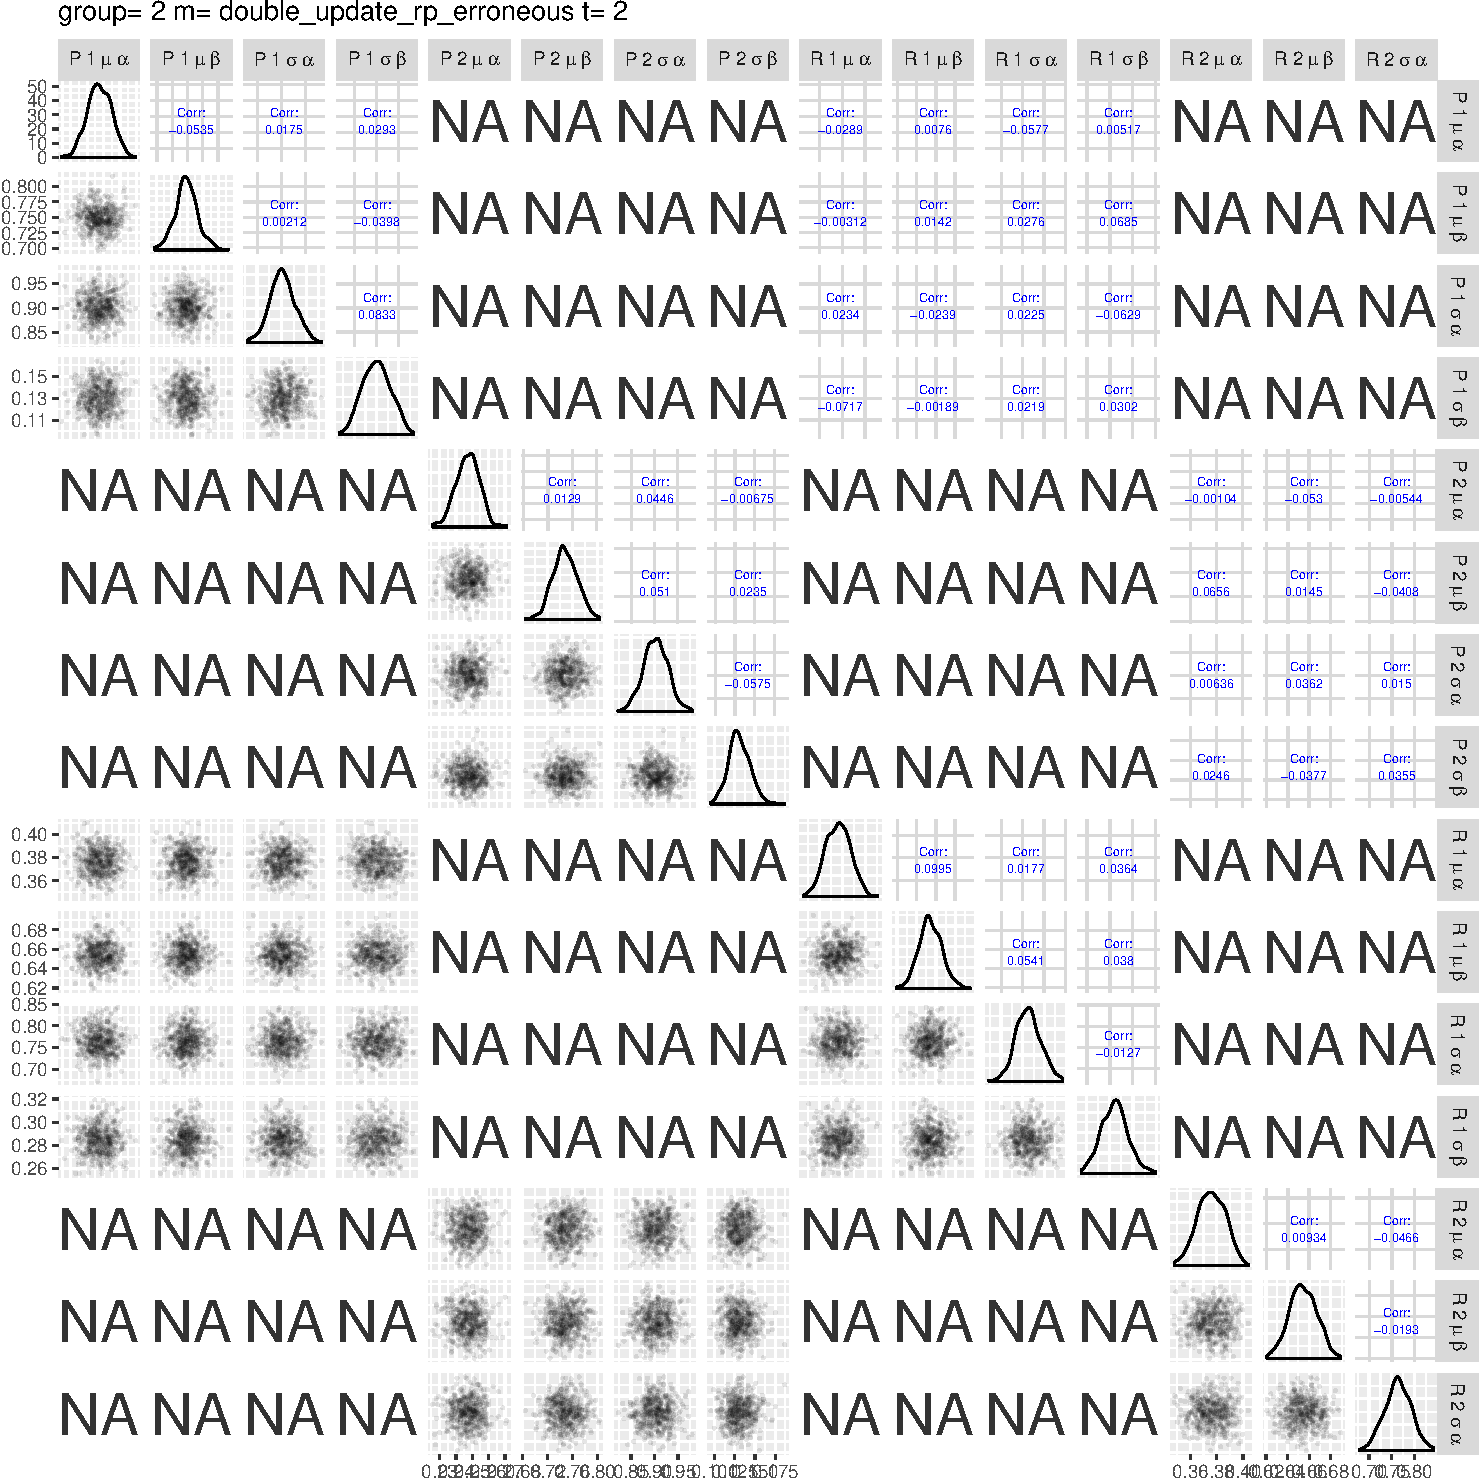
\includegraphics{compare_models_files/figure-latex/PairsPlots-8.pdf}
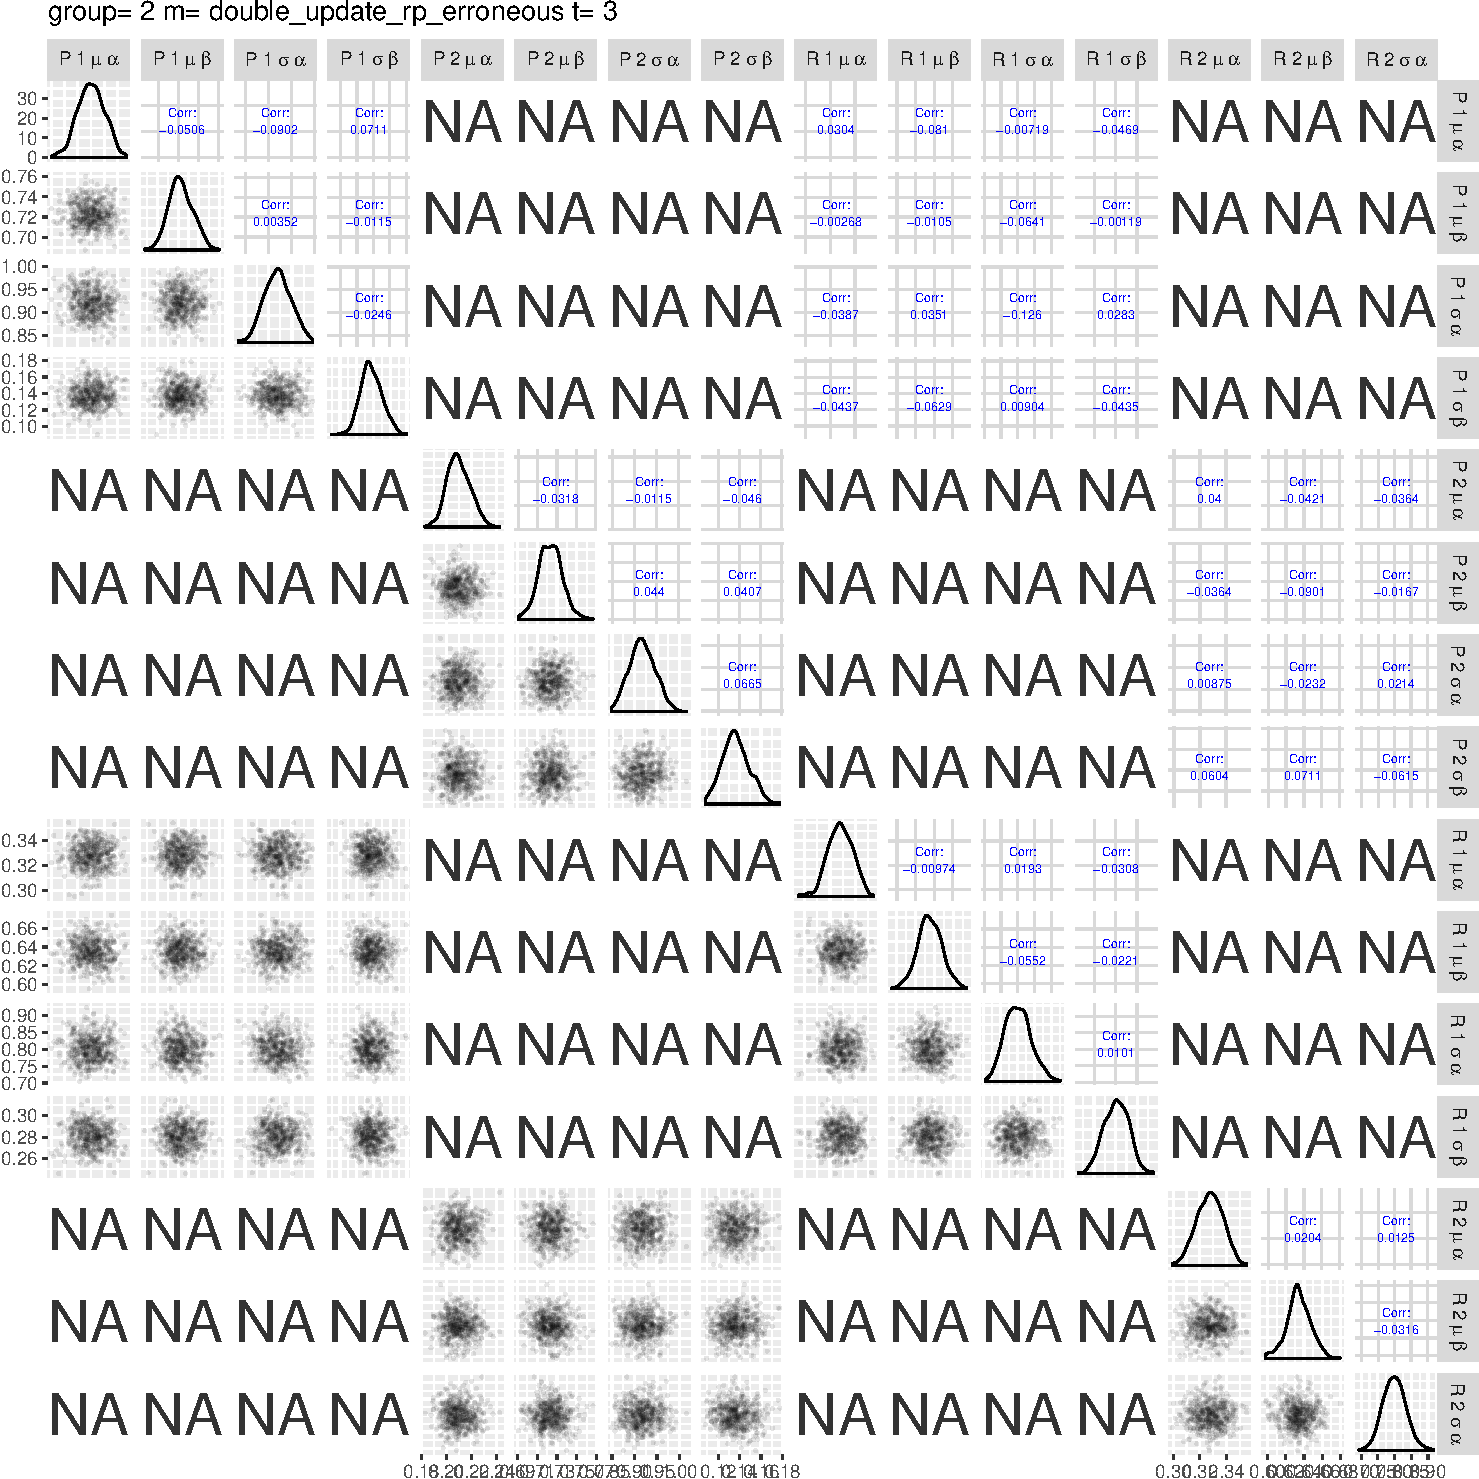
\includegraphics{compare_models_files/figure-latex/PairsPlots-9.pdf}
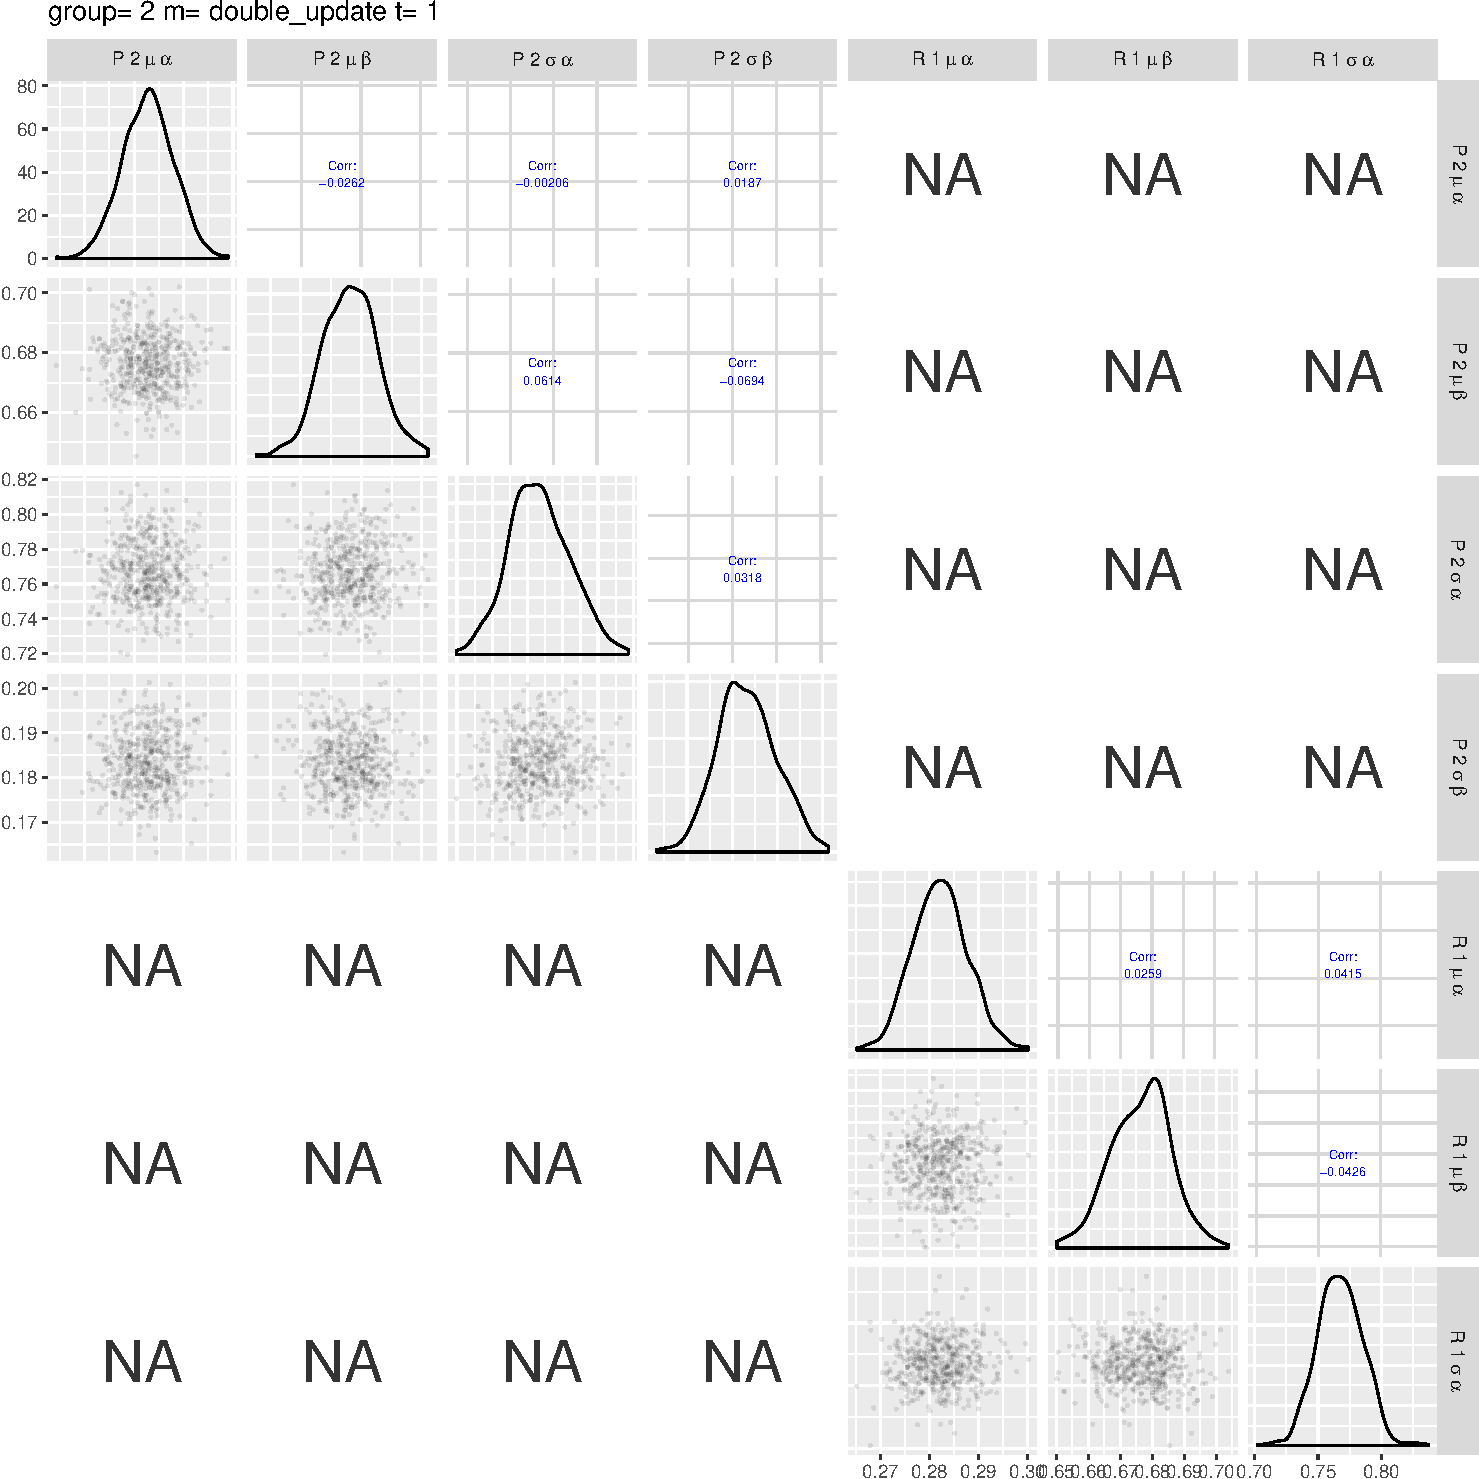
\includegraphics{compare_models_files/figure-latex/PairsPlots-10.pdf}
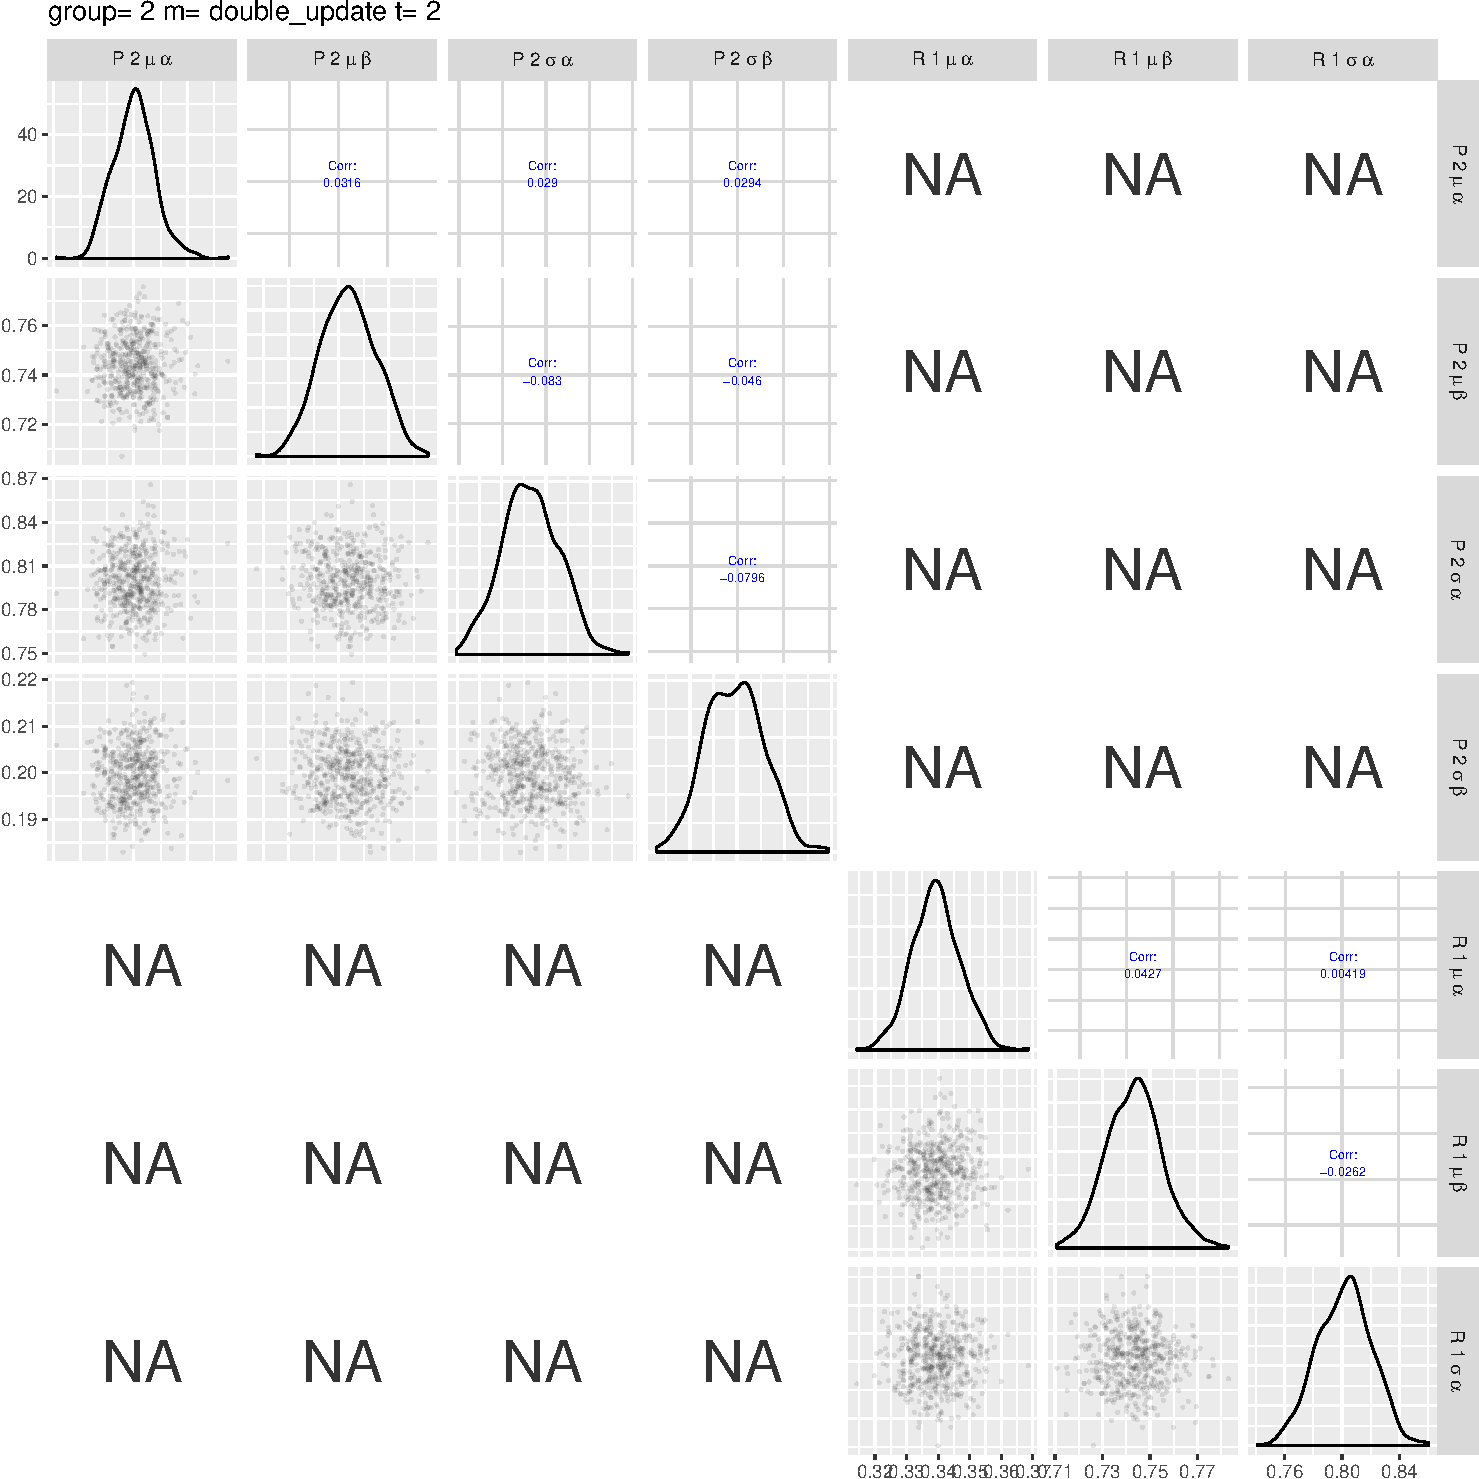
\includegraphics{compare_models_files/figure-latex/PairsPlots-11.pdf}
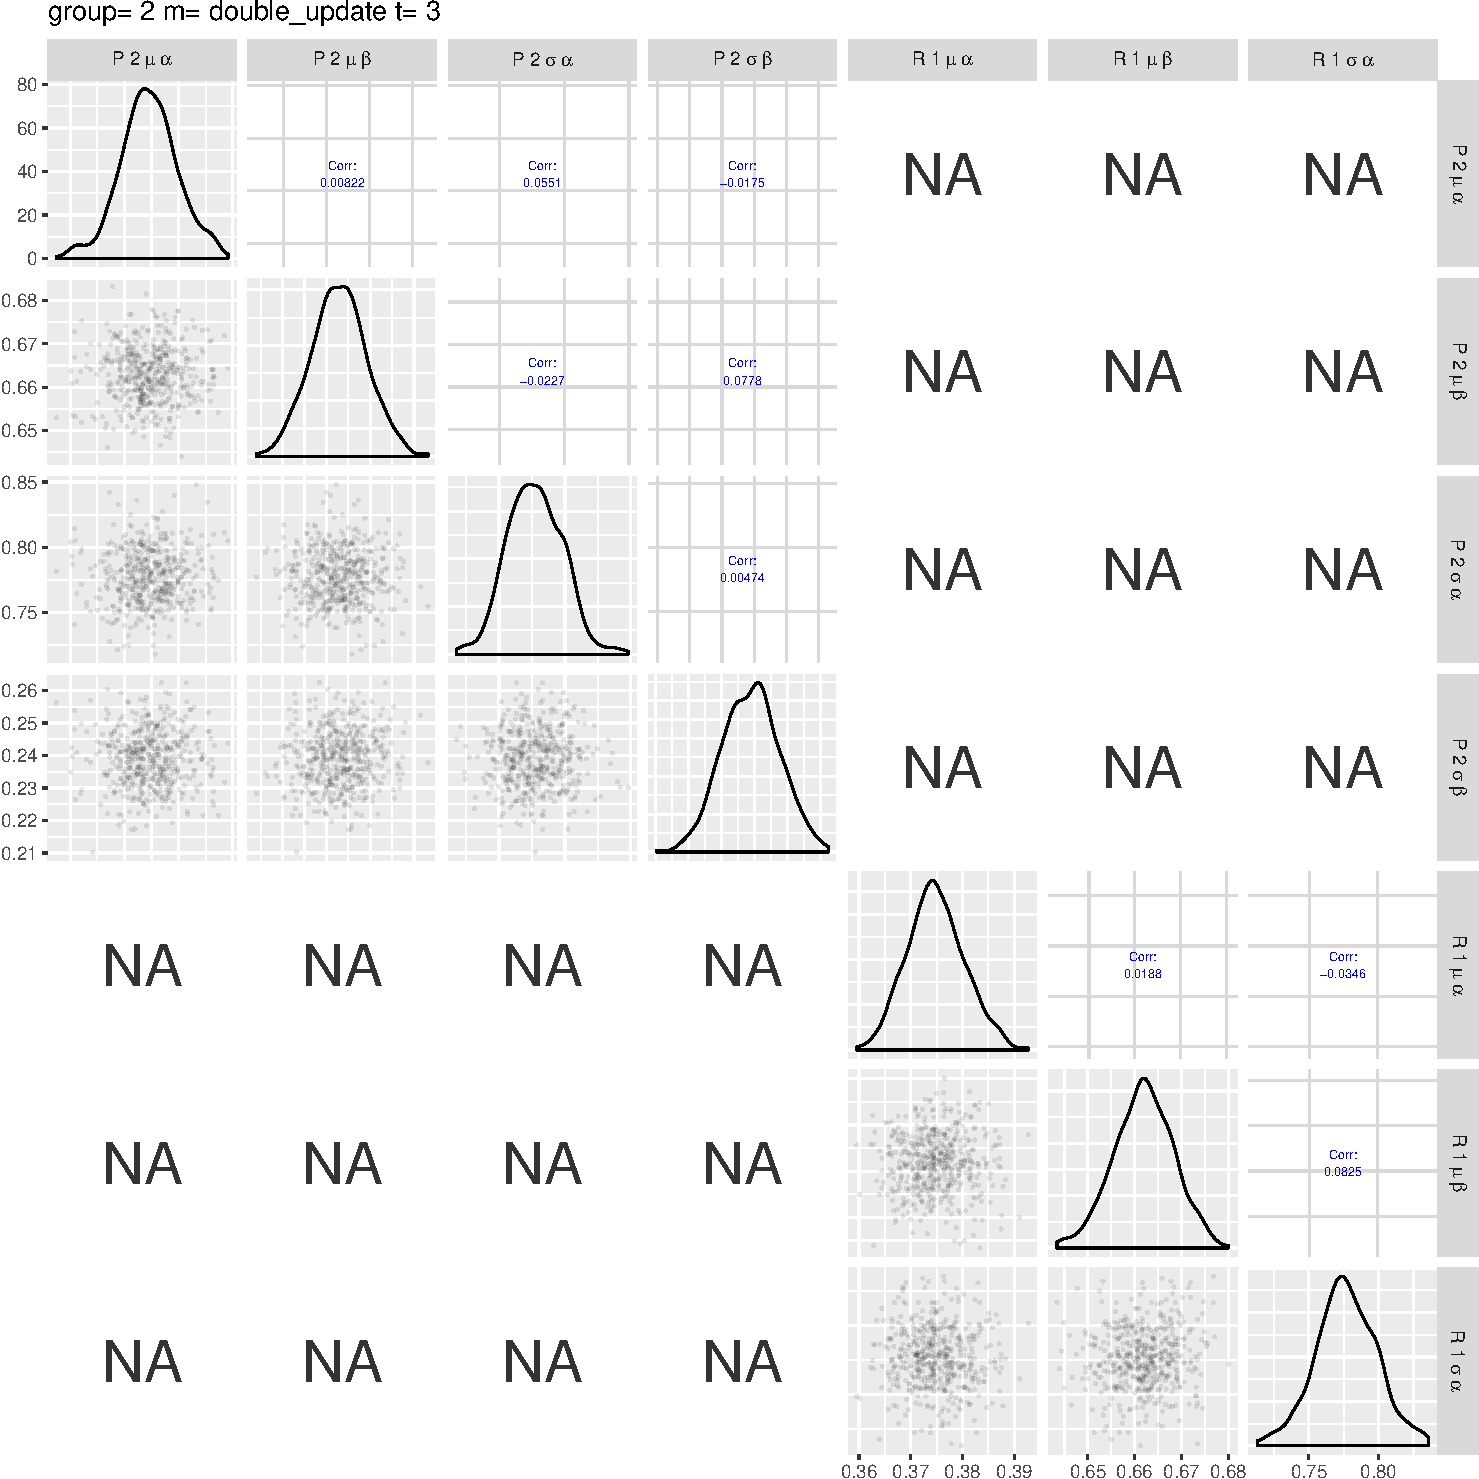
\includegraphics{compare_models_files/figure-latex/PairsPlots-12.pdf}
\includegraphics{compare_models_files/figure-latex/PairsPlots-13.pdf}
\includegraphics{compare_models_files/figure-latex/PairsPlots-14.pdf}
\includegraphics{compare_models_files/figure-latex/PairsPlots-15.pdf}
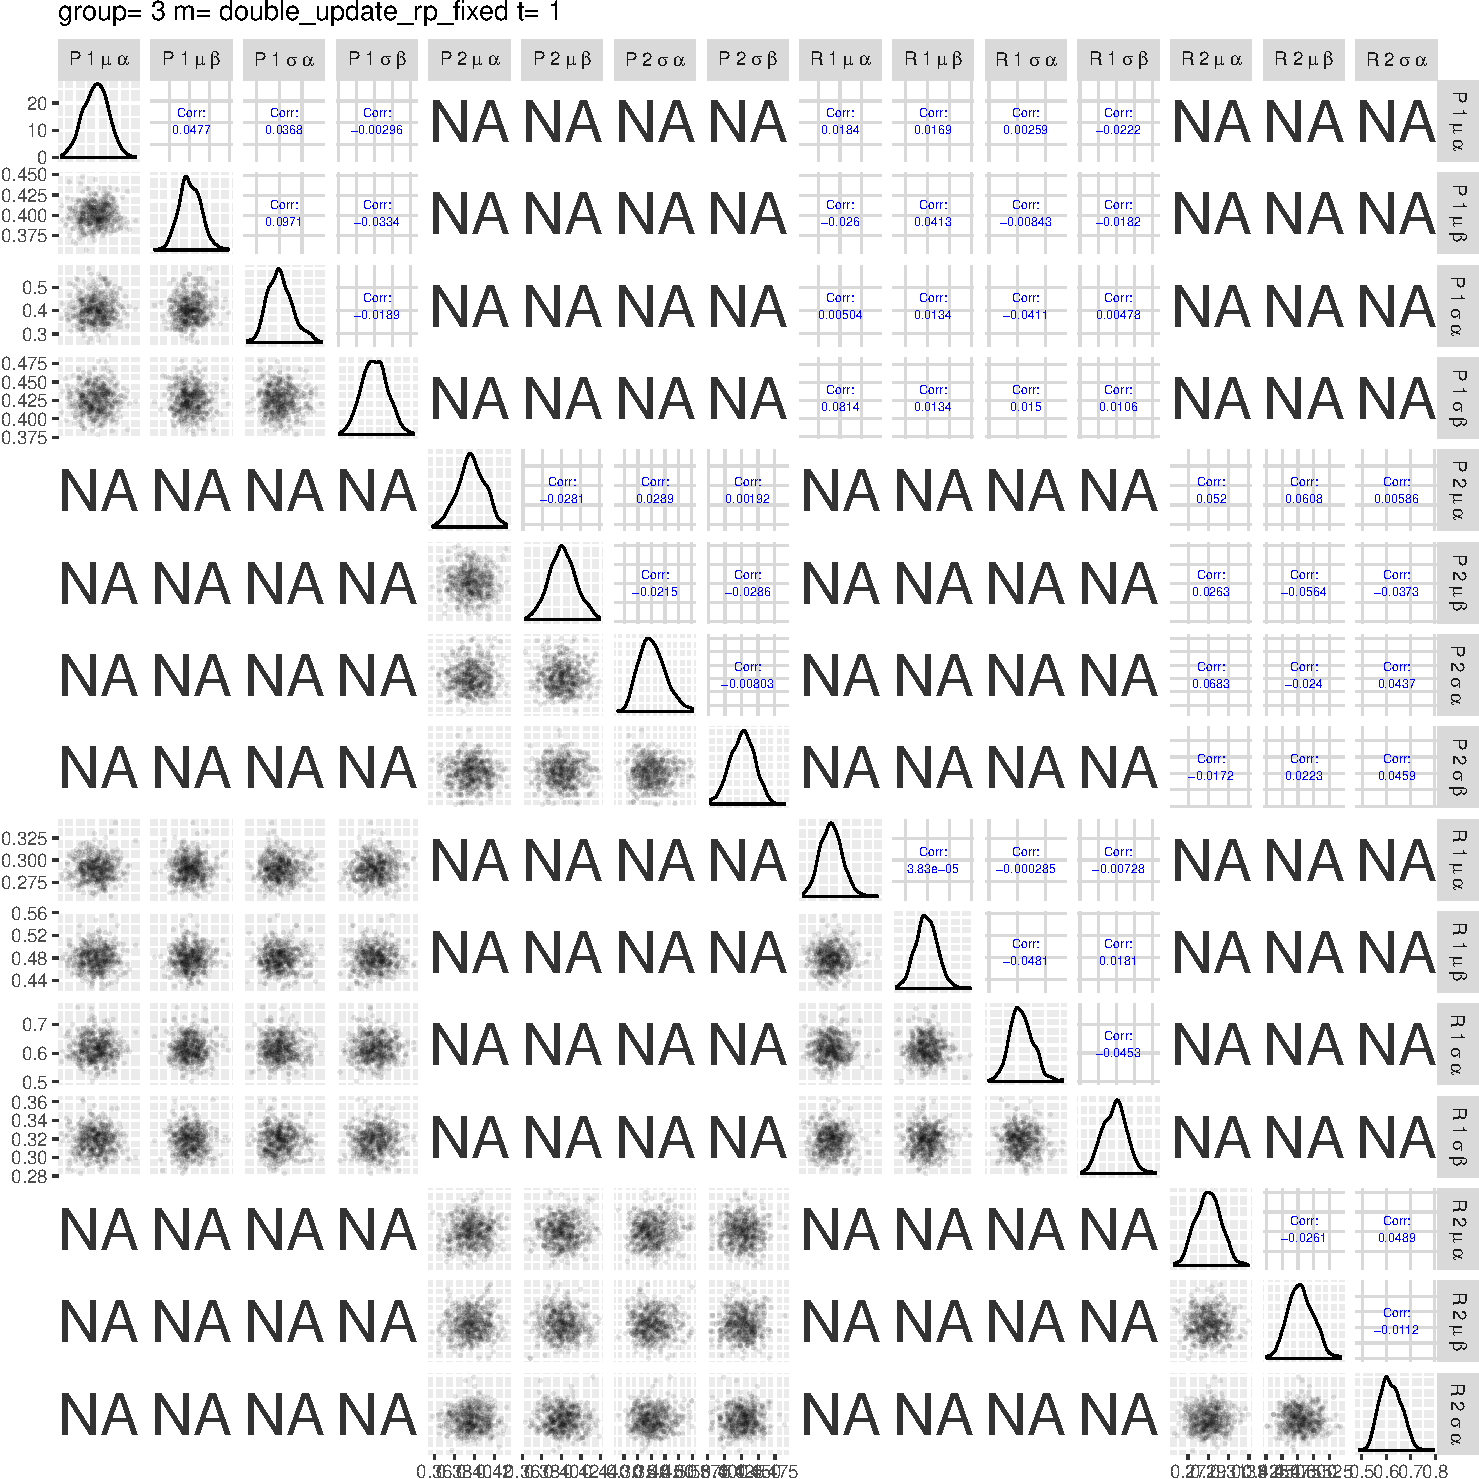
\includegraphics{compare_models_files/figure-latex/PairsPlots-16.pdf}
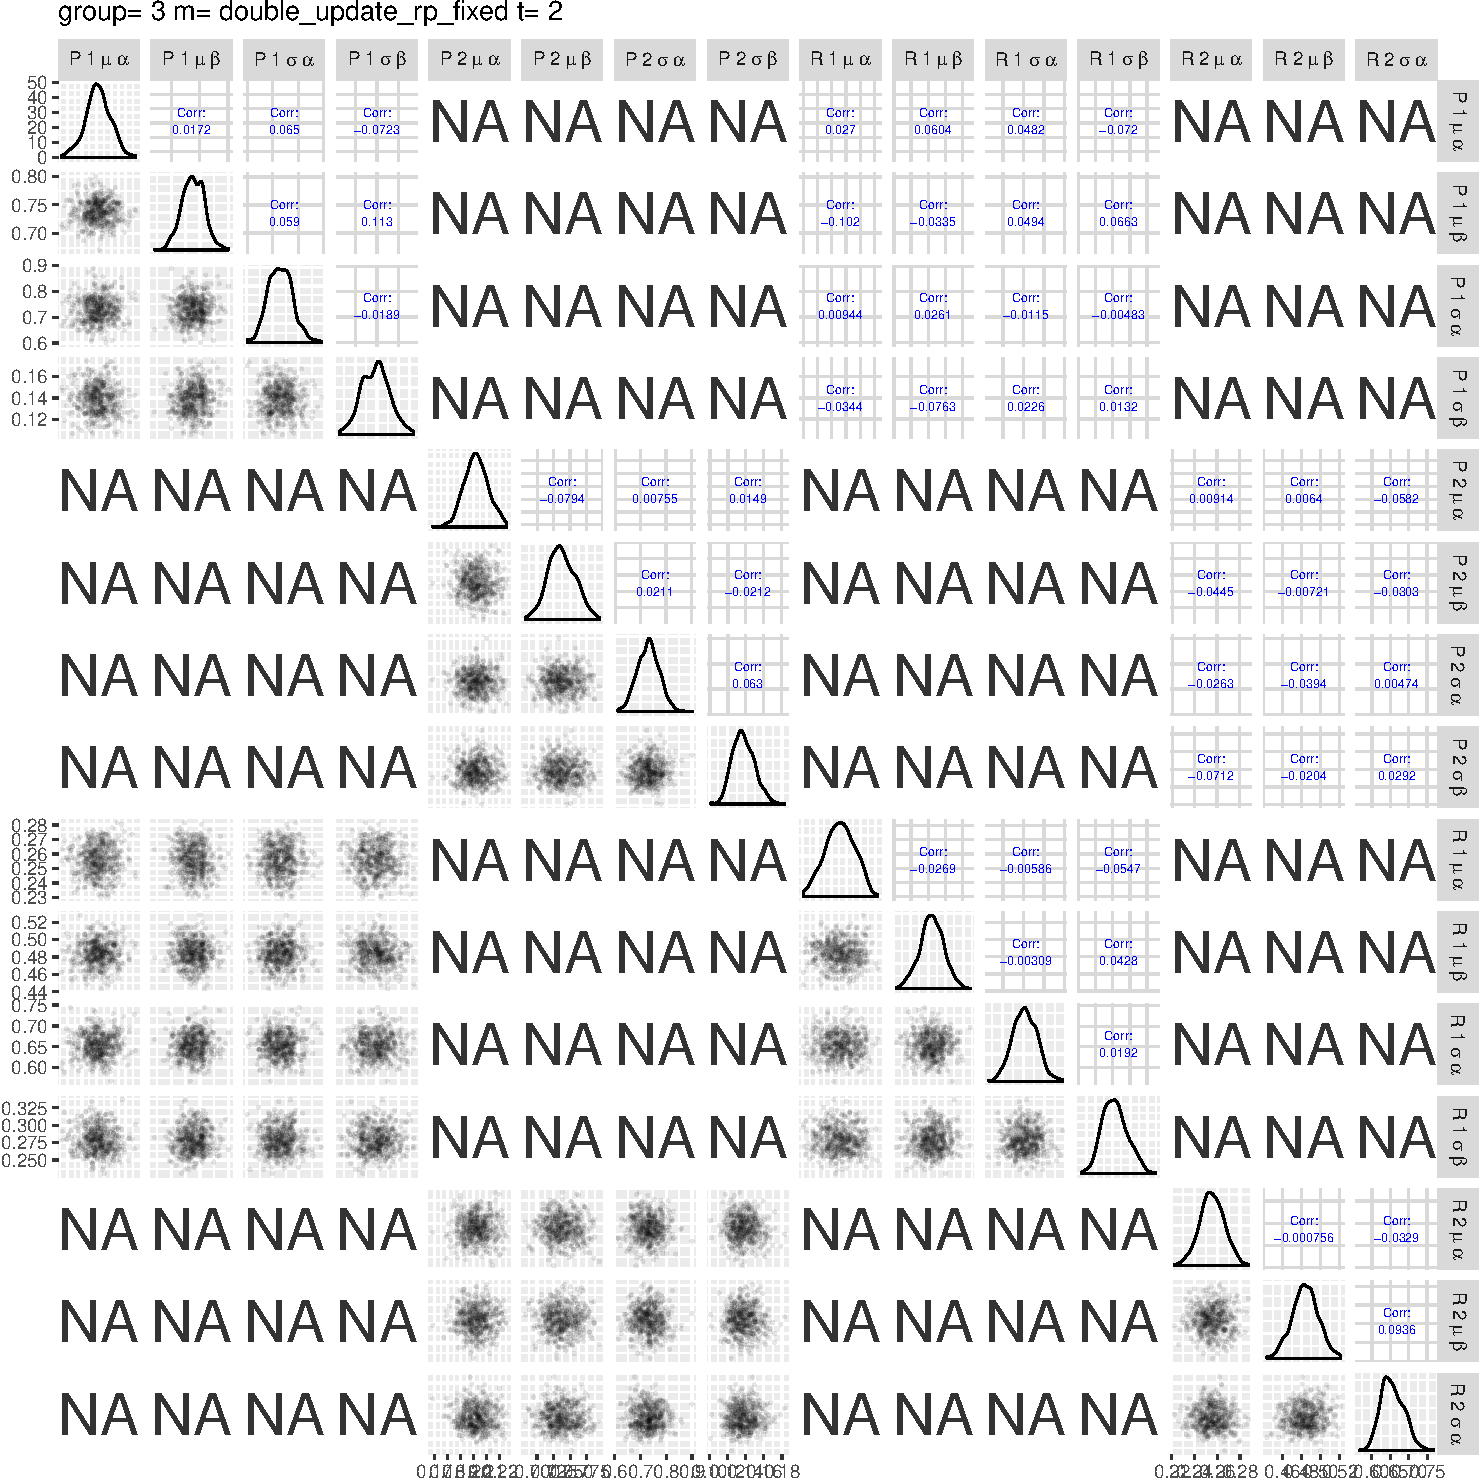
\includegraphics{compare_models_files/figure-latex/PairsPlots-17.pdf}
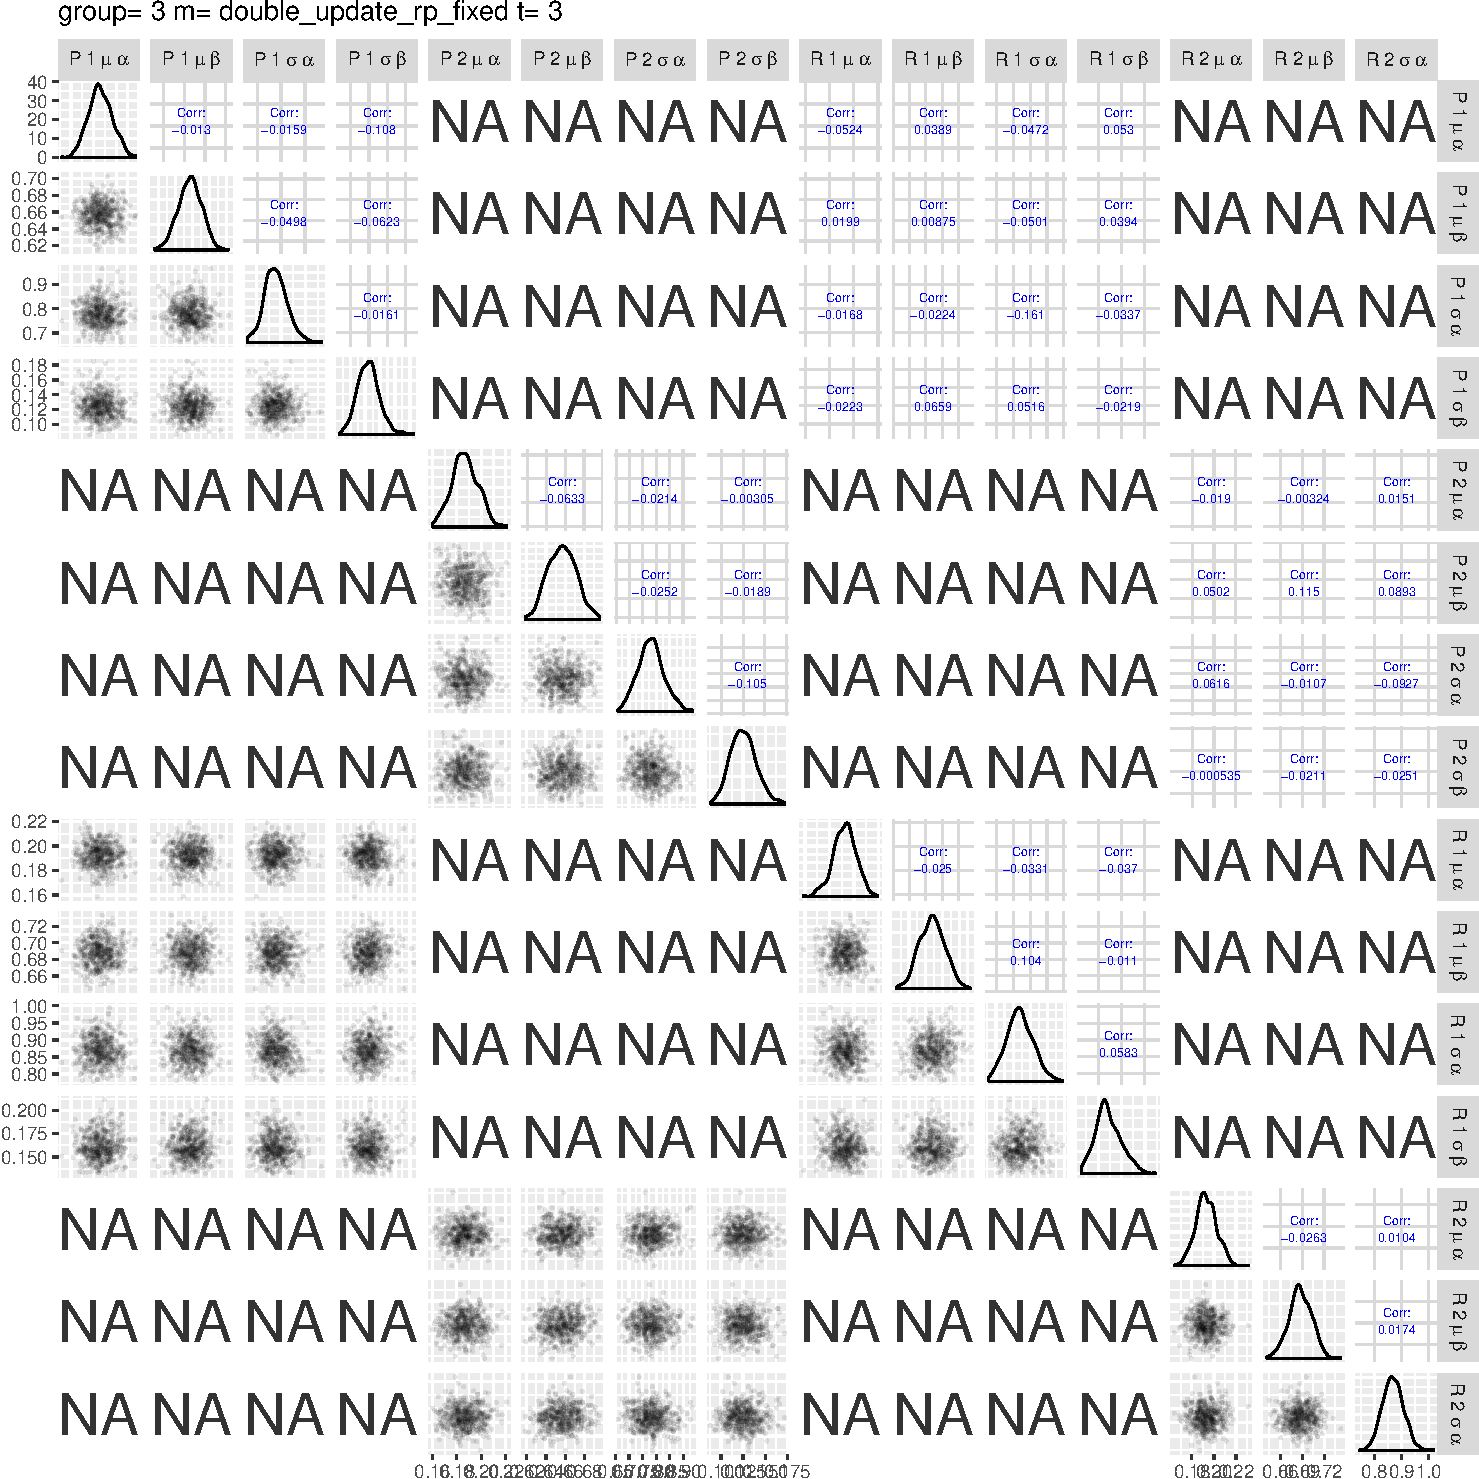
\includegraphics{compare_models_files/figure-latex/PairsPlots-18.pdf}
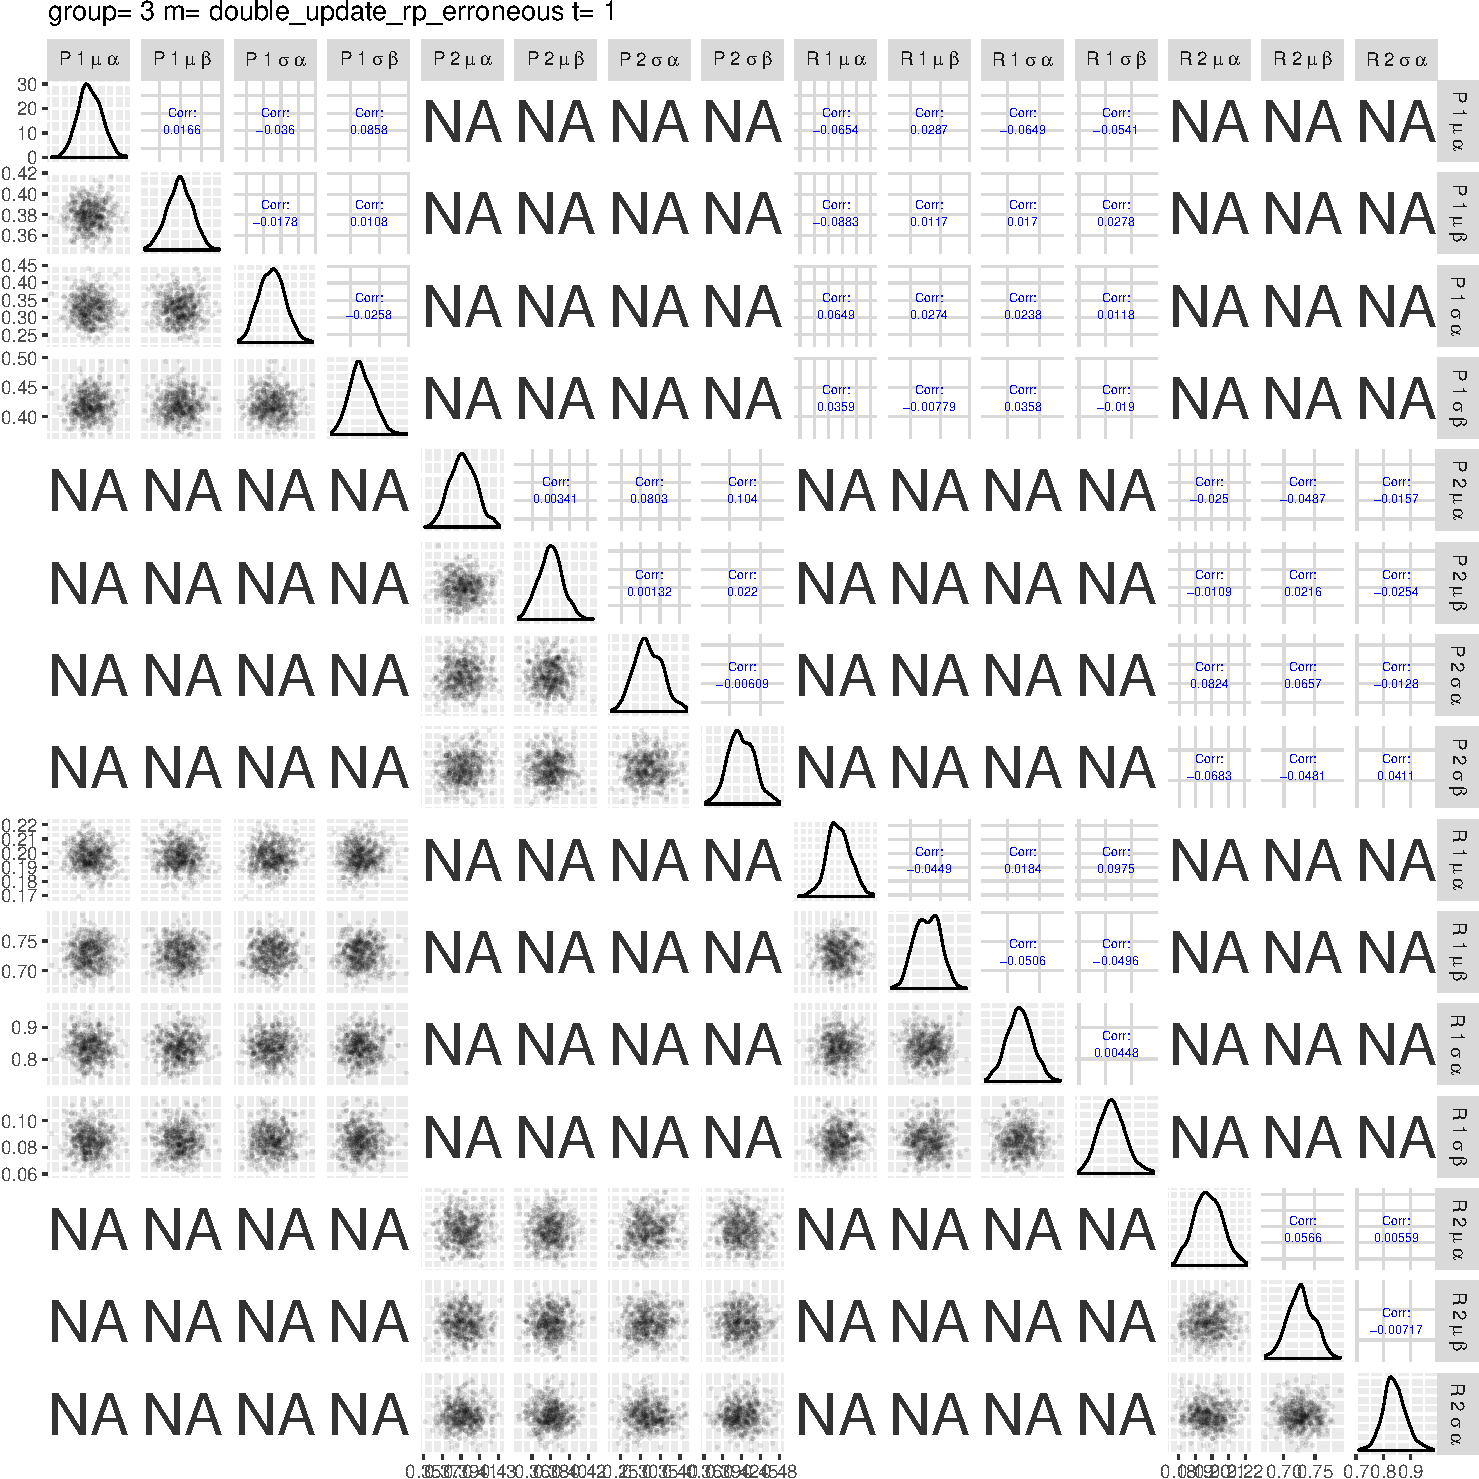
\includegraphics{compare_models_files/figure-latex/PairsPlots-19.pdf}
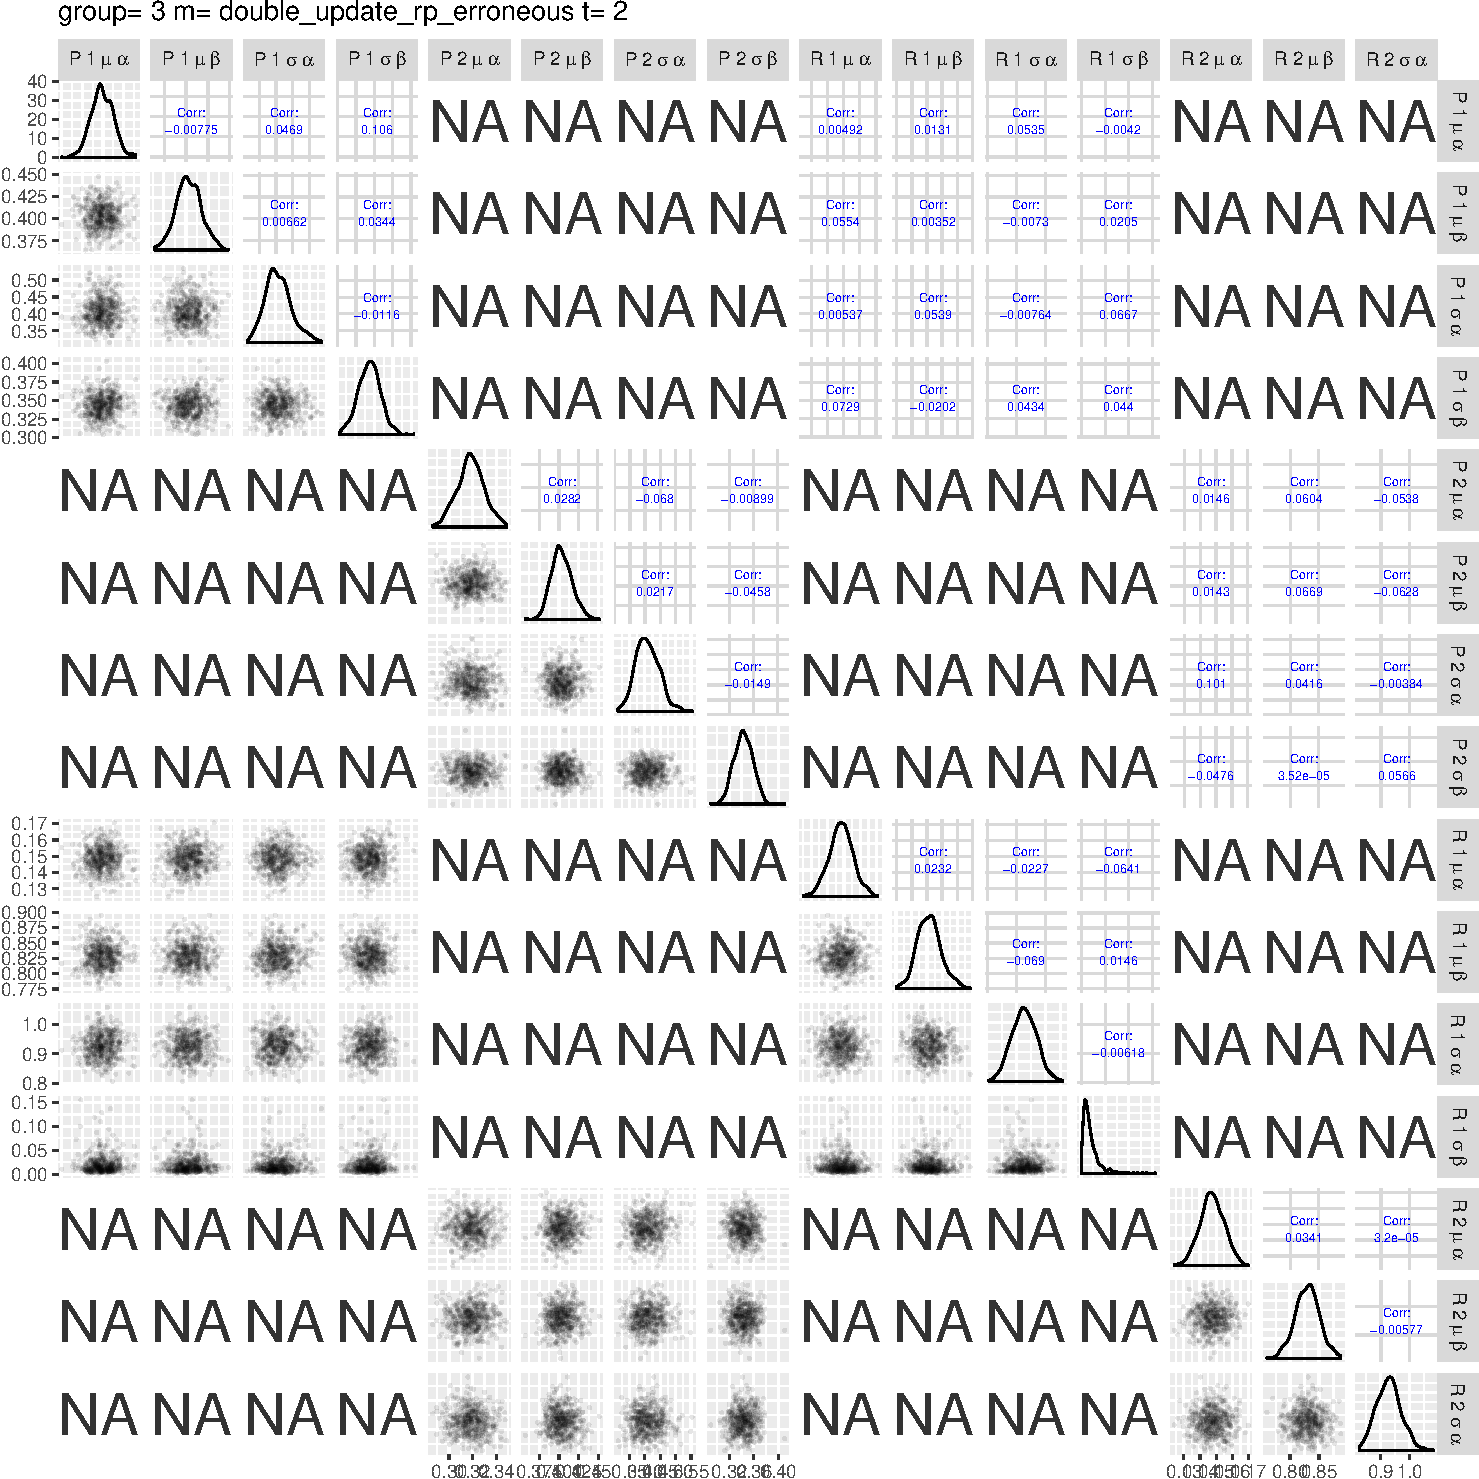
\includegraphics{compare_models_files/figure-latex/PairsPlots-20.pdf}
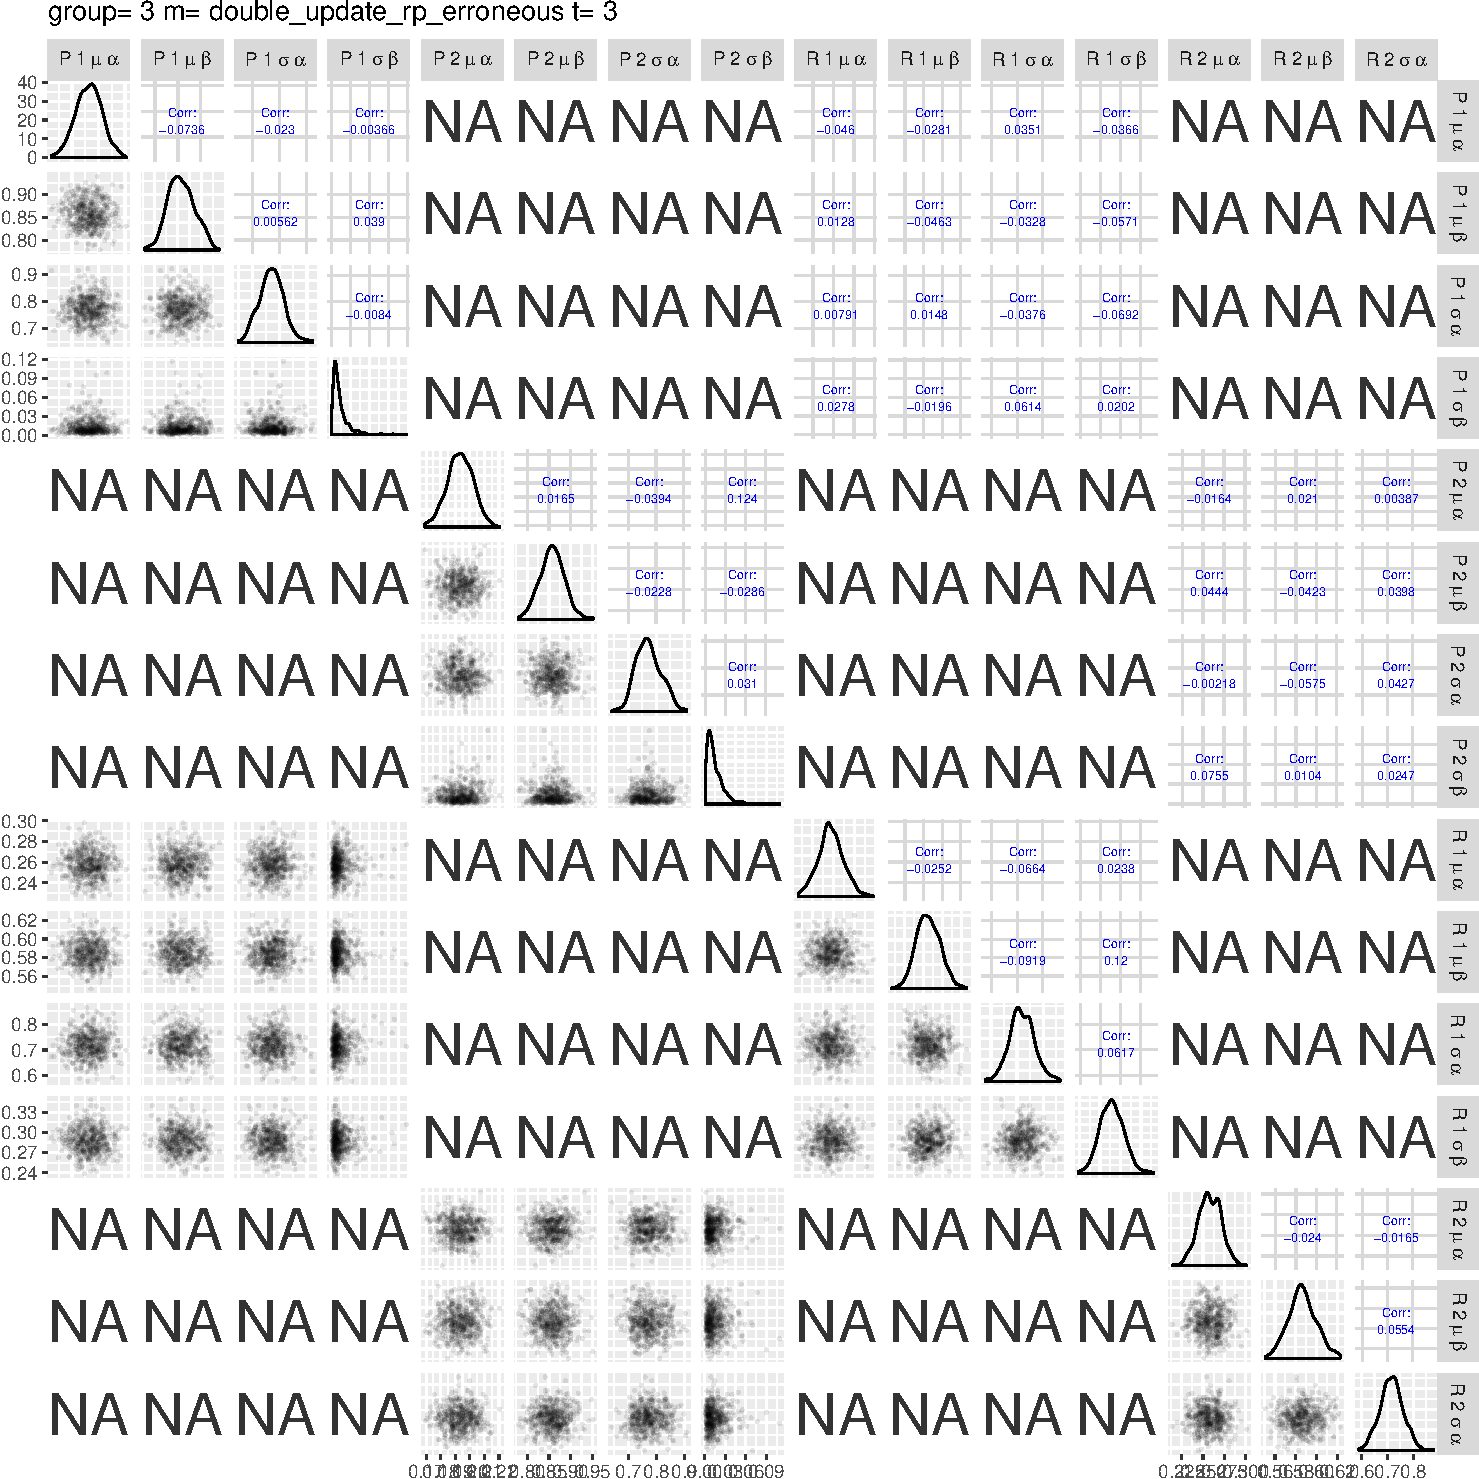
\includegraphics{compare_models_files/figure-latex/PairsPlots-21.pdf}
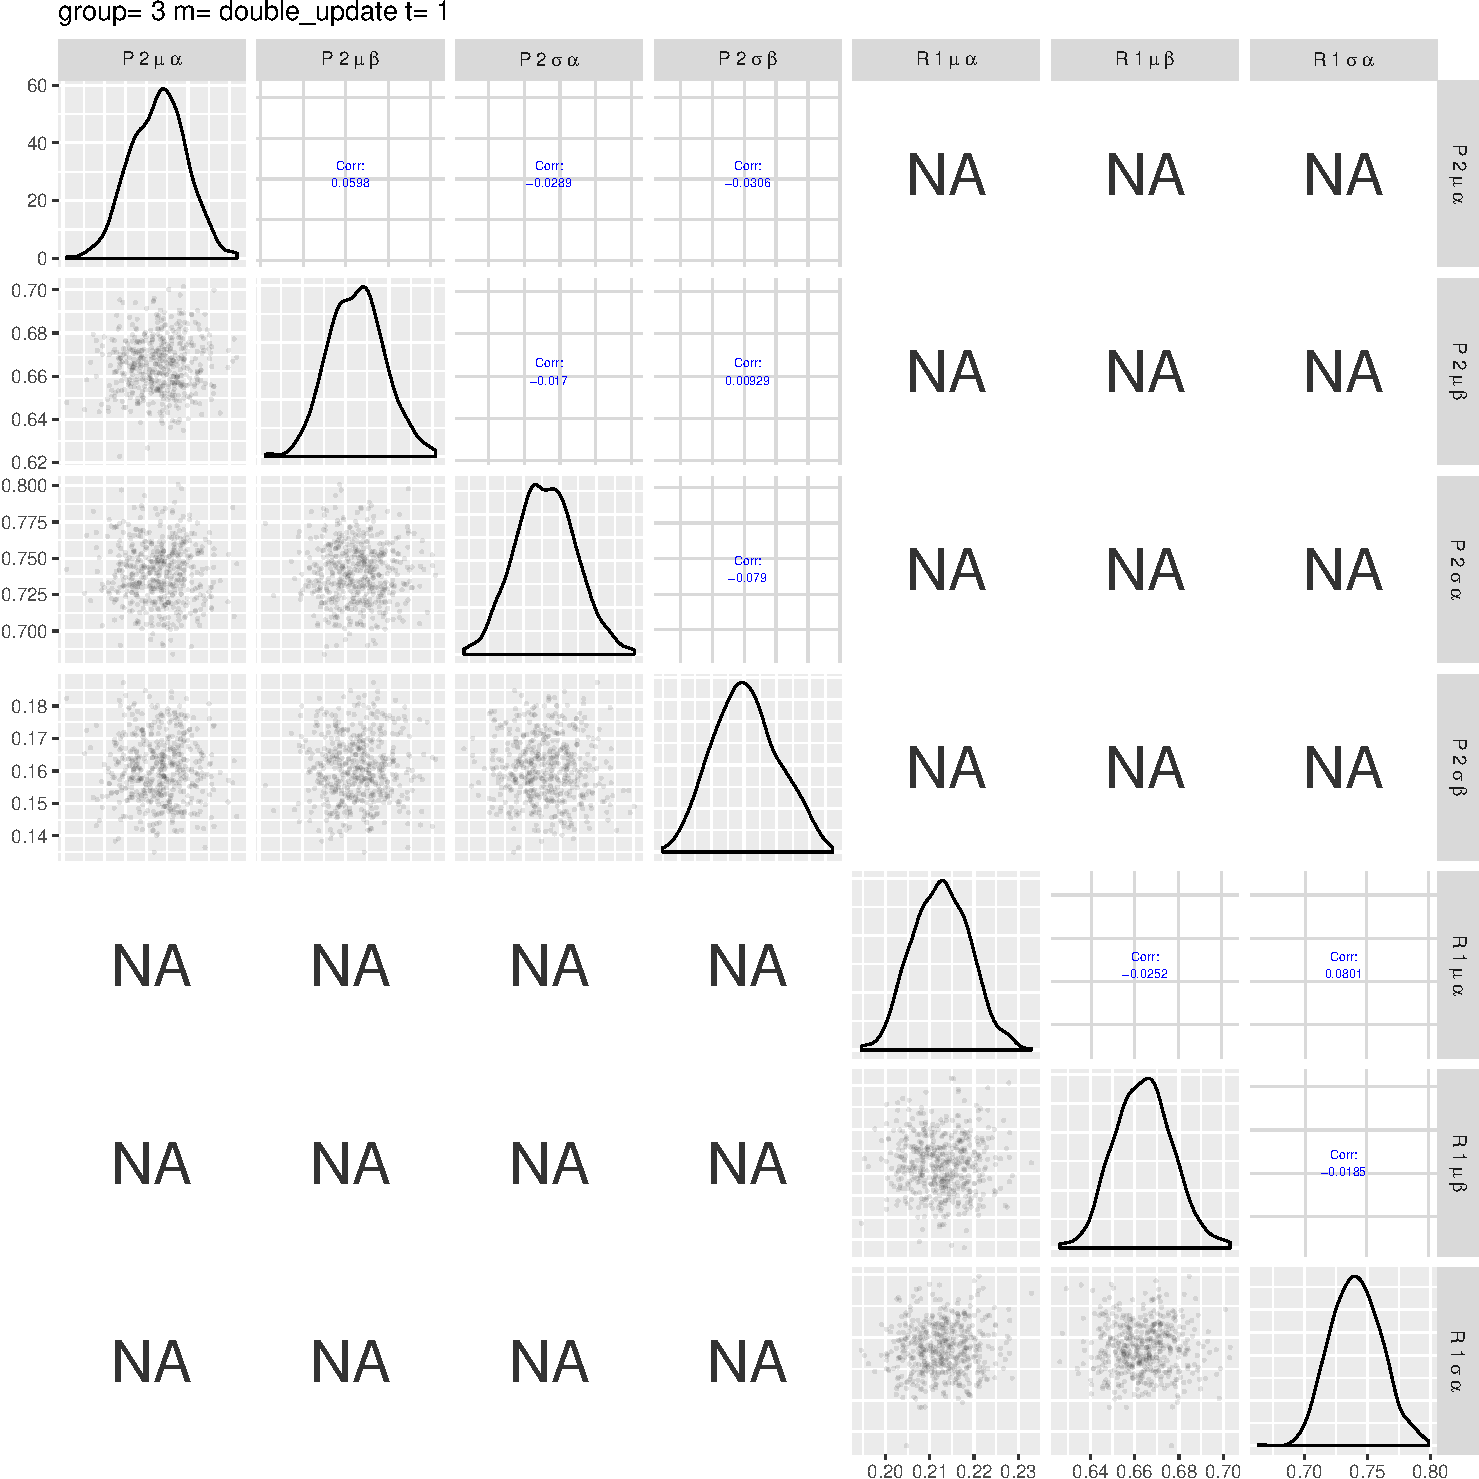
\includegraphics{compare_models_files/figure-latex/PairsPlots-22.pdf}
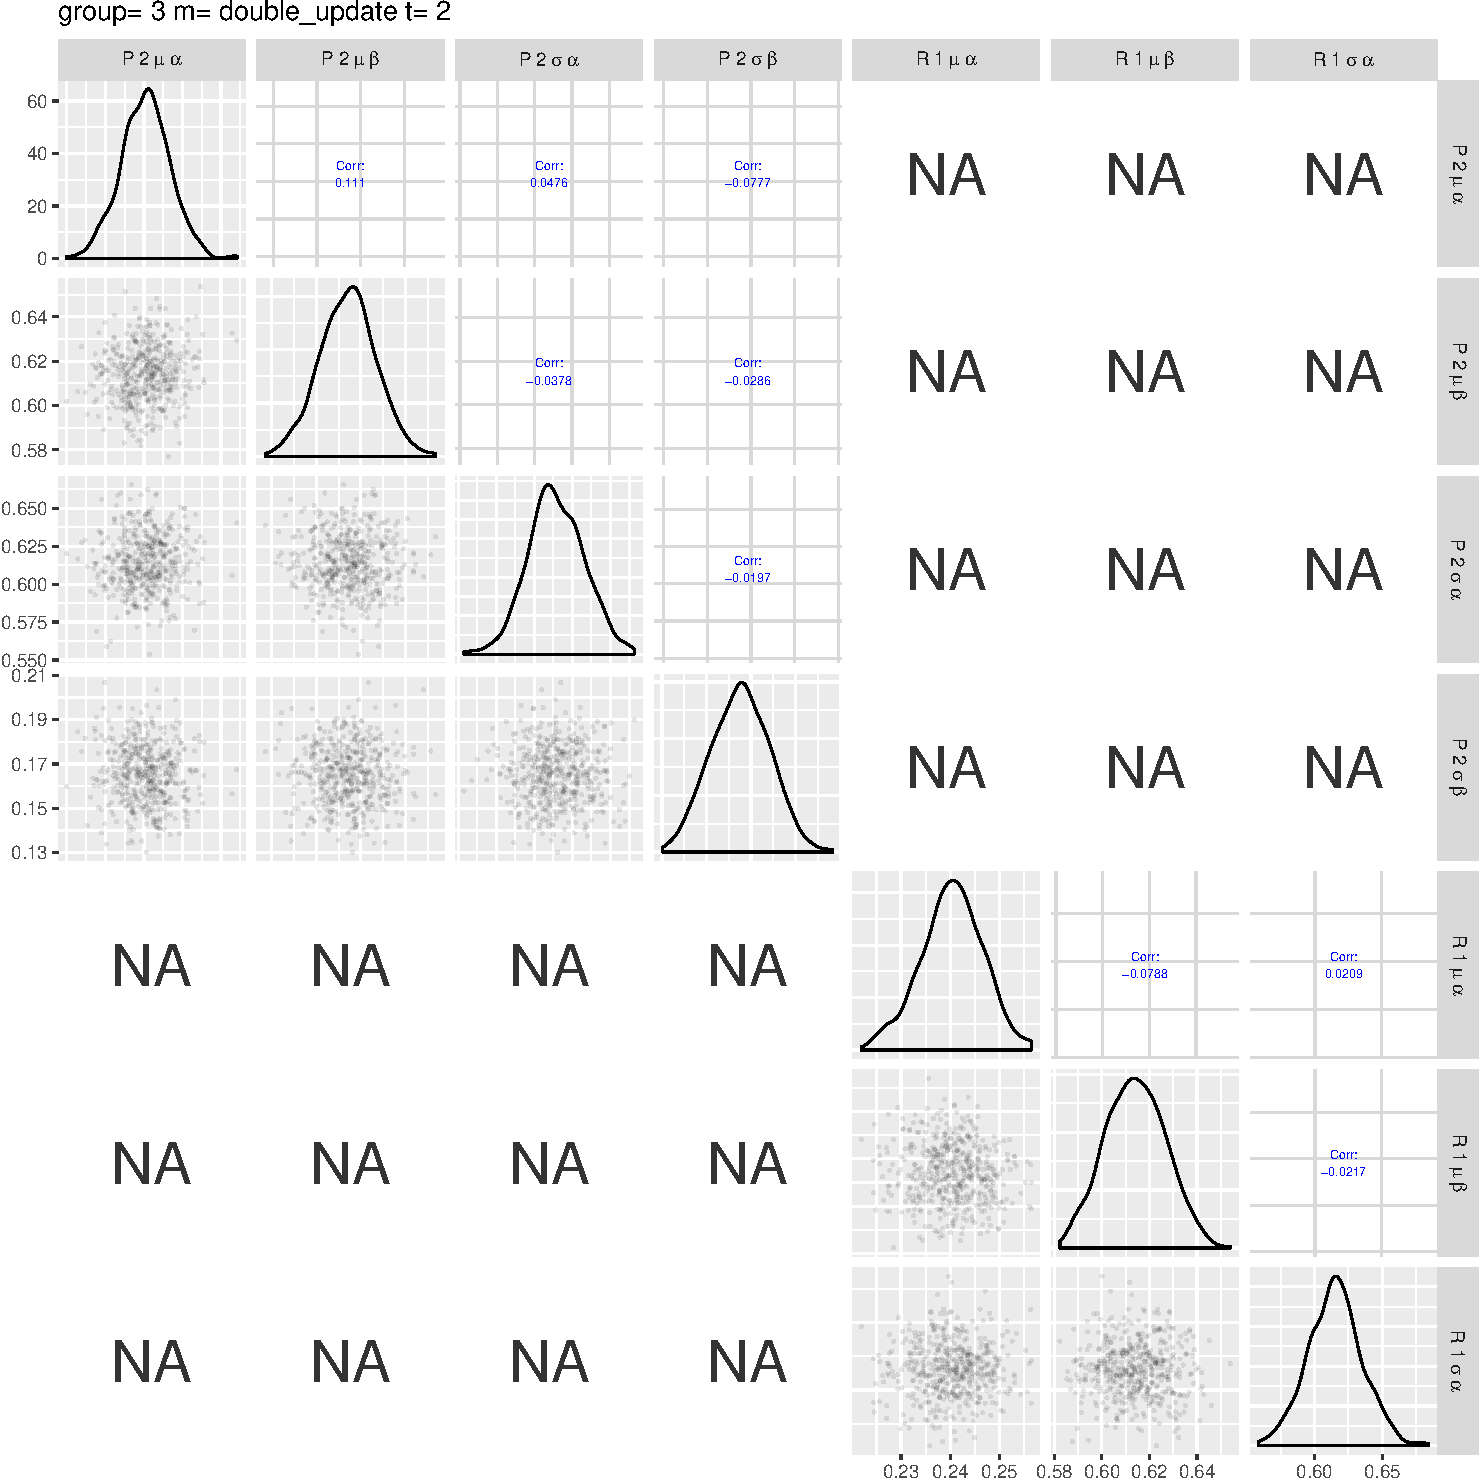
\includegraphics{compare_models_files/figure-latex/PairsPlots-23.pdf}
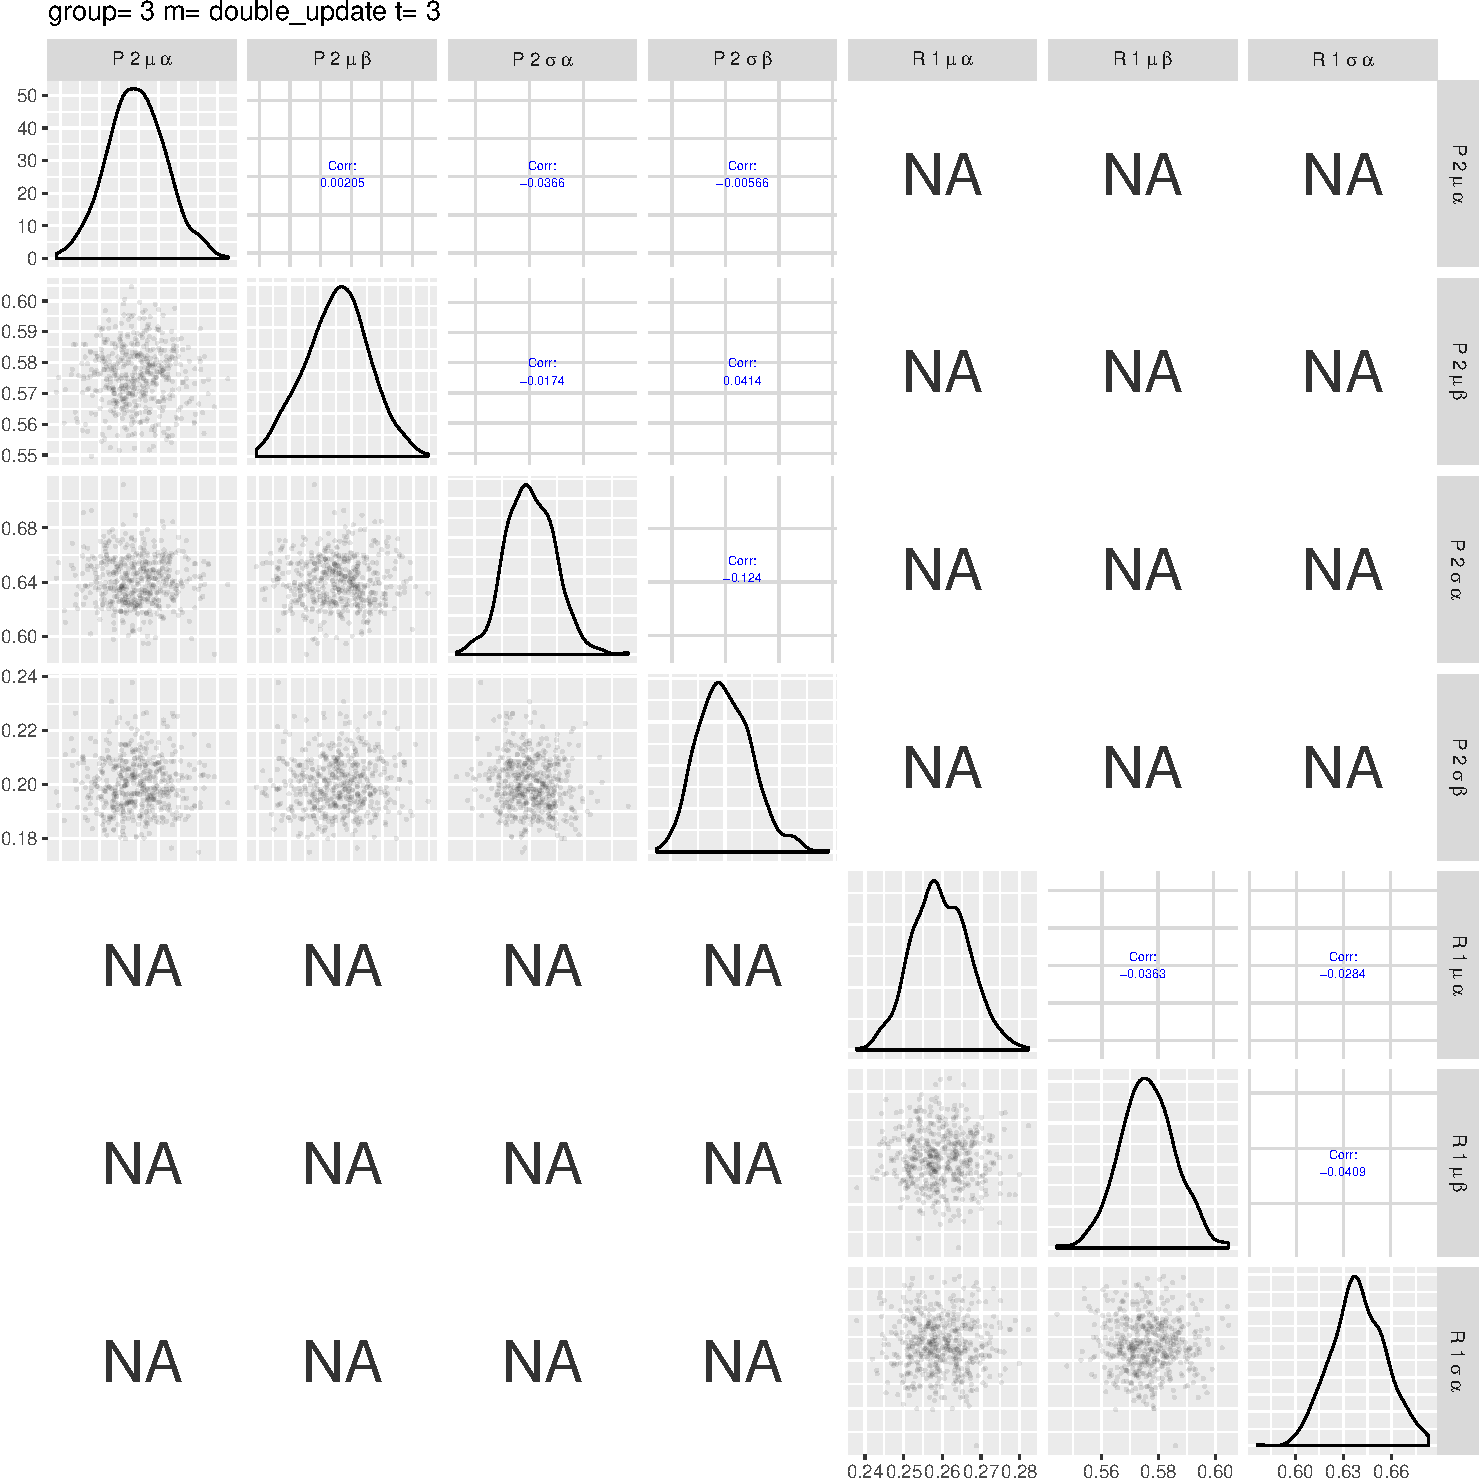
\includegraphics{compare_models_files/figure-latex/PairsPlots-24.pdf}

\section{Discussion}\label{discussion}

\(\beta\) values are reasonably consistent between repeated trials. But
for our final and most comprehensive analysis, variational bayes varies
widely between concluding that there is a real between-group difference
and that there is not.

Thus, to really get at a decent answer we will want to take a look at
using an MCMC estimator.


\end{document}
